\newcommand\showchange{FL}%{TT FL}%
\documentclass[preprint,10pt]{sigplanconf}
\usepackage{times}
\usepackage{graphicx}
\usepackage{tabularx}
\usepackage{subfigure}
\usepackage{color}
\usepackage{xcolor}
%\usepackage{caption}
%\usepackage{subcaption}
\usepackage{multirow}
%\usepackage{cite}	% sort citation numbers
\usepackage{url}
\usepackage{xspace}
%\usepackage[compact]{titlesec}
%\usepackage{amsmath}


%%%%%%%%%%%%%%%%%%%%%%
% Select one or other if want to see comments.
% \com is sometimes displayed during draft.
\long\def\com#1{}
%\long\def\com#1{{\bf \sc comment: }{\small [#1]}{\bf \sc\ endcomment}\newline}

\long\def\xxx#1{{\bf XXX: }{\small [#1]}}
%\long\def\xxx#1{}

%\if\showchange
%\usepackage[usenames,dvipsnames]{color}
%\newcommand\bluet[1]{\color{blue}{#1}}
%\newcommand\redt[1]{\textcolor{red}{#1}}
%\else
%\newcommand\bluet[1]{#1}
%\newcommand\redt[1]{#1}
%\fi

% Use this macro to force page breaks where ugly widows/orphans occur;
% be sure to recheck all uses after any significant change to the text!
\def\widowpage{\pagebreak}

% Choose abbreviated or long-version alternatives in paper
\long\def\abbr#1#2{#1}			% abbreviated version
%\long\def\abbr#1#2{#2}			% long version

% Choose abbreviations or long names/titles in bibliography
\def\bibbrev#1#2{#1}			% short version
%\def\bibbrev#1#2{#2}			% long version
%\def\bibbrev#1#2{\abbr{#1}{#2}}		% follow abbr macro

% Abbreviated or full citation lists: \abcite{basic}{others}
\newcommand{\abcite}[2]{\abbr{\cite{#1}}{\cite{#1,#2}}}

% Conference abbreviations: \bibconf[Nth]{SOSP}{Symposium on ...}
\newcommand{\bibconf}[3][]{#1 \bibbrev{#2}{#3 (#2)}}

% Stuff to eliminate for blind review
%\newcommand{\blind}[1]{#1}		% non-blind
\newcommand{\blind}[1]{}		% blind
%%%%%%%%%%%%%%%%%%%%%%

\newcommand{\kn}[1]{\texttt{\small #1}} % key name
\newcommand{\kw}[1]{{\em #1}}        	% keyword
%\newcommand\code[1]{{\scriptsize \textsf{#1}}}
\newcommand\codet[1]{{\small \textsf{#1}}}
\newcommand\code[1]{{\small \textit{#1}}}
\newcommand\ie{{\em i.e.,}\xspace}             % i.e.
\newcommand\eg{{e.g.,}\xspace}             	% e.g.
\newcommand\myds{{\bf\em{SMR}}\xspace}
\newcommand\myth{{\bf\em{Sthread}}\xspace}
\newcommand\mydsname{({\bf\em s}calable {\bf\em u}nbounded {\bf\em m}ulticast {\bf\em C}hannel)\xspace}
\newcommand\Oflag{{\tt O}\xspace}
\newcommand\Pflag{{\tt P}\xspace}
\newcommand\Wflag{{\tt W}\xspace}

\newcommand{\grayt}[1]{{\color{gray} #1}}
\newcommand{\redt}[1]{{\color{red} #1}}
\newcommand{\bluet}[1]{{\color{blue} #1}}




\title{\vspace{-5pt} SMR: A good scalability MapReduce for Multicore Systems\\
  
	\vspace{-5pt}}
\authorinfo{}{}{}
\iffalse
\authorinfo{# \and }
	{University of Science and Technology of China}
	{yufeny@ustc.mail.edu.cn}
\fi
\iffalse
\conferenceinfo{'11,} {July 11-12, 2011, Shanghai, China.}
\CopyrightYear{2011}
\crdata{978-1-4503-1179-3/11/07}
\clubpenalty=10000
\widowpenalty=10000
\fi
\begin{document}

\maketitle

\begin{abstract}
Although the multicore chips have been widely used, utilizing multicore sources is still  a challenging task due to the difficulties of parallel programming.
Traditional parallel programming techniques,  Pthreads and OpenMPI,  require programmers to manually manage many details, such as synchronization, load balance.
%solve many details of design challenge.
%The programmers need to manually manage many details, such as synchronization, load balance, by using the traditional parallel programming techniques. 
%while designing and implementing efficient, simply parallel programming model is challenging because of many details of design challenges.
%Traditional parallel programming techniques like Pthreads and OpenMPI leave programmers solving many details of design challenge.
By automatically managing concurrency, MapReduce, a simple and elegant programming model, alleviate the burden of programmer. 
Phoenix, a MapReduce library for multicore and multiprocess, demonstrates that applications written with MapReduce framwork get competitive scalability and performance in comparison to those written with Pthreads.
%Nevertheless, implementing such runtime systems for large-scale, shared-memory systems can be challenging.
%And it shows that MapReduce is a promising model for scalable performance on mulitcore and multiprocess.
%And applications written with MapReduce framwork have competitive scalability and performance comparied to those written with Pthreads.
However, evaluation results show that the optimized Phoenix \cite{yoo2009phoenix2} scales worse on an 4-chip, 32-cores system running x86 Linux.

This paper focuses on improving Phoenix in terms of scalability and performance.
First, we analyze some important roadblocks that limit scaling of the Phoenix runtime on shared-memory systems.
%we analyze the limitations of scalability and performance. 
Then, a novel thread library \myth is proposed, which is well scalable for multicore. 
Based on \myth, we design a modified  MapReduce model \myds, which use a new producer-consumer model is used to pipeline Map and Reduce phase.
%MapReduce library, \myds, which is based on a scalable thread library, \myth.
Finally, we evaluate \myds on a 32 CPU cores processor and the result demonstrates that  applications, like \codet{histgram}, \codet{word\_count} and \codet{pca}, can achieve 
better scalability and performance than Phoenix.
%up to speedup over Phoenix in term of scalability and performance.

%is a safe and efficient alternative to Phoenix. 
%In addition, evaluation results show 
%application like \textit{pca} and \textit{word\_count} have better 
%scalabiliy and performans than Phoenix. 

\end{abstract}

%\input{terms}
\section{Introduction}
\label{sec:intro}

%%需要调研的部分:解答的问题,为什么我们关注多核的scalability问题。随着分布式系统的广泛普及,企业和用户的通用的做法是通过堆积更多的机器来获取更快的处理效率和速度。但是机器堆积的越多,网络带宽,耗电也越来越多,如何充分利用单台机器的多核资源成为很重要的课题。

%一方面,随着多核机器的广泛普及,如何充分利用多核资源成为非常重要的课题,另一方面,现有的很多我们希望充分利用单台机器上的资源,

%目前的现状,需求
As the prevalence of multicore chips,
it is foreseeable that tens to hundreds (even thousands) of cores on a single chip
will appear in the near future\cite{Borkar2007core}.
While utilizing multicore sources is still challenging
because of the difficulties of parallel programming.
Specifically, the thread-based model requires the programmer to manually
manage synchronization, load balancing, and locality, which is
often error-prone (e.g., races and deadlocks) or requires detailed
understanding of the underlying hardware.
An alternative approach is to rely on a runtime system for
concurrency management. 

MapReduce\cite{dean2004mapreduce}, 
for instance, is a promising programming model for clusters
to perform large-scale data processing
in a simple and efficient way.
In most cases, programmers only need to implement two functions:
map and reduce.
The runtime system spawns multiple threads that apply
these functions concurrently across the elements of the input
dataset. 
%The runtime spawns multiple threads to worker and 
%automatically manages synchronization, load balancing, 
%and locality in order to achieve efficient execution.
%which aggregates values in the key-value pairs according to the key.
And the programmer dose no need to control synchronization 
and schedule tasks manually.
%面向多核的MapReduce的相关工作
While initially MapReduce is implemented on clusters, Ranger
et al. have demonstrated the feasibility of running MapReduce
applications on shared memory multicore machines with 
Phoenix\cite{ranger2007phoenix}.
Other libraries such as Metis\cite{mao2010metis} 
, Tiled-mapreduce\cite{chen2010tiled} and MRPhi\cite{lu2013mrphi}, 
also show that MapReduce is a promising programming model 
for multicore platforms to take full advantage of  
processing resources.
Phoenix uses the pthread library to assign tasks 
among CPU cores and relies on
shared memory to handle inter-task communications.

%Phoenix存在的问题,scalability较差的原因
This work focuses on improving Phoenix\cite{ranger2007phoenix}'s scalability and performance.
On the one hand, 
While the original Phoenix performed well on small-scale systems,
we found that the runtime significantly underperformed on large-scale systems with multicores.
Specially, the performance will be better 
when the number of cores increases from 1 to 4, 
while the performance will be worse if using more than 4 cores. 
On the other hand,
there is a strict barrier between the Map and the
Reduce phase, which is bad for pipeline and hardware resource utilization.
To achieve scalable performance while retaining
the simplicity of the runtime-based approach, 
it becomes crucial to address these issues.

In contrast, Phoenix is a shared-memory version of
MapReduce targeted for multi-core and multiprocessor systems.
Phoenix uses shared-memory threads to implement parallelism
Ideally, adding more threads and cores to the runtime
would bring about a linear decrease in execution time.
However, the benefits of adding more
cores will be reduced due to overhead associated with the
additional threads----the contention of lock.
Due to parallel programming model is shared-memory multithreading, 
where all threads of an application share a single address space. 
%A common parallel programming model is shared-memory multithreading, 
%where all threads of an application share a single address space. 
This shared address space has a
cost, which will limit the scalability of these applications. 
%All of these operations are synchronized by a single per-process lock. 
Hence, with the continuously increasing
number of cores, it can easily cause resource pressures on the
runtime, operating systems and the CPU caches, 
which could significantly degrade the performance. 

%Compared to the cluster version, MapReduce on multicore is able to take ad-
%vantage of fast inter-task communications in shared memory, thus
%avoids the expensive network communications among tasks.

%我们如何解决这个问题
%为了改进Phoenix存在的这些问题,我们提出了一个scalable mapreduce库,它即具有较好的性能,且具有较好的scalability.
To remedy the above problems, 
firstly, we propose a Scalable thread libray(\myth).
Then this paper presents a modified model of \myds(Scalable MapReduce), 
that can efficiently support MapReduce applications.
\myds reserves the similar Phoenix programing interfaces as well.
Specifically, this paper make the following contributions:(\redt{need talk more....})
\begin{itemize}
  \item We identify the important roadblocks 
  that limit scaling of the Phoenix runtime on shared-memory systems. 
  Specifically, we find that shared address space
   becomes a crucial issue at large thread counts.

  \item We demonstrate the approach with the \myds runtime using a 32-cores system. The optimized runtime exhibits significantly improved scalability over the
original system; For 32cores, the new runtime improves speedup by **× 
(maximum improvement of speedup up to **×).

  \item We aim at providing an race-free programming abstraction to
support scalable MapReduce.
  \item We present a scalable MapReduce.
\end{itemize}

%介绍文章的组织结构
In order to ground our discussion, we present an overview
of MapReduce architecture and Phoenix in Section 2. 
We then develop the design of \myth in Section 3, 
keeping the focus on the implementation mechanism of extention. 
%In Section 4 we show how \myth can support
%\myds and illustrate
%the potential benefits of that producer-consumer model for MapReduce framework.
In Section 4 we describe our support for pipelineing map and reduce,
and illustrate the potential benefits of that producer-consumer model for MapReduce framework. 
We present initial performance results in Section 5. 
Related and future work are covered in Sections 6 and 7.

%This paper is organized as follows. In section 2, we review
%the background. Section 3 briefly describes the problems.
%Section 4 presents the experimental setup. Section 5 discusses
%the results in terms of execution time and total power
%consumption. Finally, Section 6 concludes the paper.

\section{Background}
\label{sec:back}
In this section, we will review the MapReduce programming
model and detail the salient features of Phoenix, 
an implementation of MapReduce for multicore.
Then the limitation of Phoenix in the aspect of performance is analyzed.
%讨论Phoenix的局限与不足

\subsection{MapReduce Programing Model}
Inspired  by funnctional languages, the MapReduce programming model is proposed for data intensive computation in cluster environment.
Its simple programming interface requires programmer to  define only two primitives: map and reduce.
The map function is applied on the input data and produces a set of intermediate key-value pairs.
The reduce function is applied on all intermediate pairs and  groups them with the same key to a single key-value pair. 
In order to save networking bandwidth and reduce memory consumption, the combine function, an optional operation, can aggregate the key-value pairs locally in Map phase.


The charm of MapReduce is that, for applications that can adapt, it hides all the concurrency details from  programmer. 
For example, one can count the number of occurrences for each word in a text file. 
The map function emits a $\langle word, 1\rangle$ pair for each word in document, and the reduce function counts all occurrences of a word as the output. 
The combine function is similar to the reduce function, but only processes a partial set of key-value pairs in Map phase.


\subsection{Phoenix}
Phoenix is an implementation of MapReduce for multicore  and multiprocessor systems using Pthreads.
It shows MapReduce model is a promising model, and the applications written with MapReduce have competitive scalability and performance in comparison to those written with Pthreads\cite{ranger2007phoenix};
Phoenix stores the intermediate key-value pairs produced 
by the map workers in a global matrix (Figure \ref{fig:phoenix:intermediate}). 
Each map and reduce workers can write or read this global matrix. 
%Concurrent map workers can touch the same area without synchronous controls.
When map and reduce workers operate the matrix concurrently,
two strategies must be carried out to avoid lock contention costs.
\begin{itemize}
	\item Each row of the matrix is exclusively used by a map worker, and each column of the matrix is exclusively used by a reduce worker. 
%	\item There is a barrier between the Map and Reduce phase. After all map workers have been completed, the reduce workers begin to compute. 
	\item There is a barrier between the Map and Reduce phase. Only when all map workers have been completed do the reduce workers begin to compute. 
\end{itemize}

\begin{figure}[!h!t]  
    \centering
    \includegraphics[width=0.45\textwidth]{eps/phoenix_intermediate.eps}
    \caption{Phoenix intermediate struct}
    \label{fig:phoenix:intermediate}
\end{figure}

By adopting above strategies, Phoenix effectively reduce lock contention costs in applications. 
However, These strategies limit the performance of Phoenix.
We will detail next Section. 

\section{Analysis of Phoenix}
%Phoenix demonstrates tha applications that fit the MapReduce model can perform competitively with parallel code using Pthreads.

%Though Phoenix has demonstrated promising feasibility when running applications on multicore, it has limitations in terms of scalability and performance due to its manners of design and implementation.
In this section, we first evaluate Phoenix built with a scalable memory allocator.
Then we will analyze the important roadblocks that limit scalability and performance of the Phoenix runtime on shared-memory systems.



\subsection{Scalability}
%We first evaluate the scalability of Phoenix built with jemalloc, a good scalable memory allocator, and than we measure the scalability of \myds to demonstrate the effectivity of \myds.
Since there are many heap objects shared among threads in Phoenix, it is sensitive to memory allocator\cite{yoo2009phoenix2}.
The memory allocator in glibc (i.e.,  ptmalloc\cite{gloger1997ptmalloc}) does not scale on multicore system, while jemalloc\cite{evans2006jemalloc} can provide improved performance and scalability. 
Therefore, we evaluate the scalability of Phoenix built with jemalloc, denoted as \codet{Phoenix-jemalloc}.

\begin{figure}[!h!t]  
	\centering
	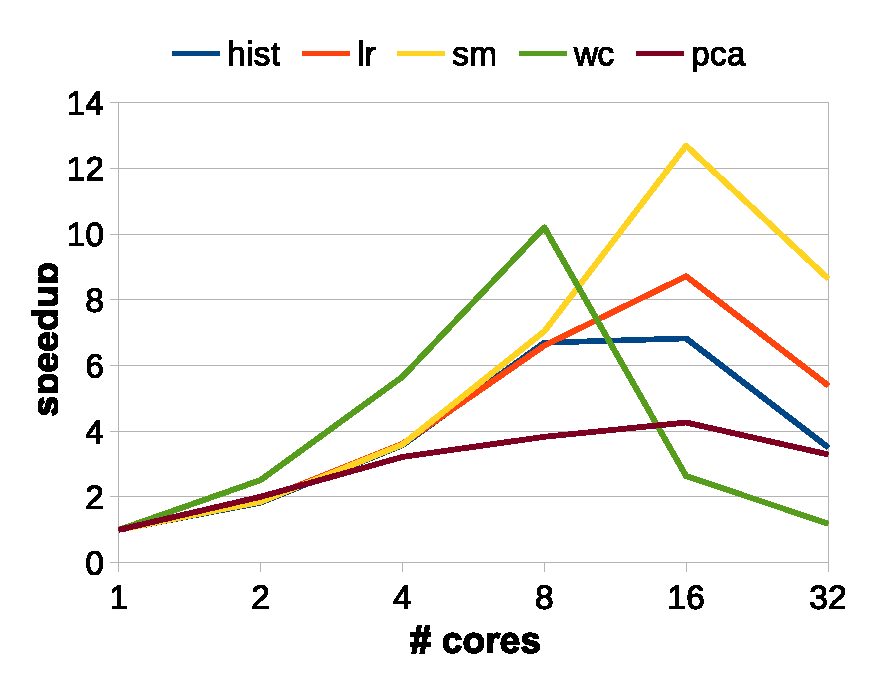
\includegraphics[width=0.45\textwidth]{eps/phoenix_speedup_jemalloc.eps}
	\caption{speedup of Phoenix-jemalloc}
	\label{fig:phoenix:speedup:jemalloc}
\end{figure}

%For linear\_regression (lr) and string\_match (sm),  using 16 or more  cores leads to speedup degradation.

Figure \ref{fig:phoenix:speedup:jemalloc} illustrates the speedup of Phoenix built with jemalloc.
We observe that applications scale well when the core count increases from 1 to 8.
However, when the core count increases from 8 to 16 to 32, the speedup sharply degrades for \codet{wc} and from 16 to 32 cores for the other applications.
The results indicate that in spite of using the scalable memory allocator, Phoenix can not scale up to 16 cores.

In order to analyze the limited scalability behavior, Linux perf is exploited to collect execution time information of hot function. 
We note that the map function is the hottest function with less cores, while \_\_ticket\_spin\_lock will become the hottest function with more cores.
\_\_ticket\_spin\_lock is a type of spinlock which is caused by the contention on the shared structure in Linux kernel.
In order to specially explore the impact of spinlock in Phoenix, we collect the execution time percent of \_\_ticket\_spin\_lock on each benchmark from 1 to 32 cores by Linux perf.

\begin{figure}[!h!t]  
	\centering
	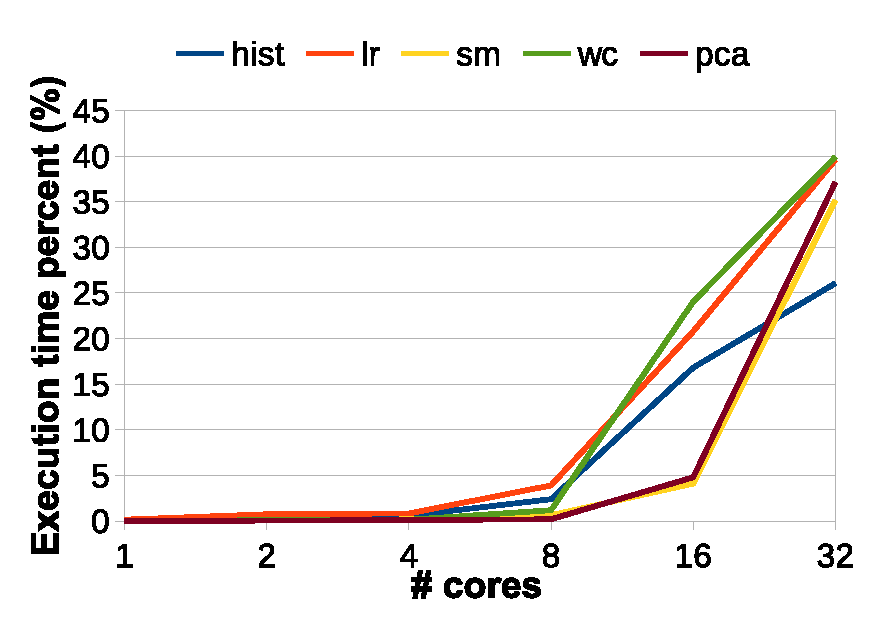
\includegraphics[width=0.45\textwidth]{eps/phoenix_spinlock_jemalloc.eps}
	\caption{speedup of Phoenix-jemalloc}
	\label{fig:phoenix:spinlock:jemalloc}
\end{figure}

As the result shows in Figure\ref{fig:phoenix:spinlock:jemalloc}, the cost of spinlock increases quickly as the cores number cross a specific value (i.e., 8).
%Specially, for hist with 16 and 32 cores, \_\_ticket\_spin\_lock is the function that has largest execution time percents of 40.15\%  and 71.25\%, respectively. 
Specially, for \codet{wc} 16 and 32 cores, \_\_ticket\_spin\_lock (i.e., spinlock) is the function that has largest execution time percents of \redt{24.04\%} and \redt{39.91\%}, respectively. 
Experiment results demonstrate that Phoenix suffers from serious lock contention when the cores number exceeds 8. 
That means most of execution time will be used for waiting but not actual computation.

%Phoenix performs well with less cores, it can not scale up 16 cores for all applications. 
%Actually, when cores number exceed 8, the speedup of \codet{wc} and \codet{hist} on Phoenix begin degrading. 

%Phoenix performs well with no more than 16 cores.
%However, when core number exceed 16, .
%For lr and sm, the speedup is degraded when cores is greater than 16.


%on \codet{hist}, \codet{wc} and \codet{pca} when the number of core is less than 8.
%As the number of cores increase (from 1 to 8), the performance of Phoenix increase for all cases, i.e., the execution time decreasing. 
%While For 16 to 32 cores, Phoenix performance keep decreasing with the increase of the number of cores.

%The above performance changes can be explained from contending on the shared address space in Linux kernel.
%Therefore, we collect \_\_ticket\_spin\_lock execution time percent information to peek the contention by Linux perf.
%The results as shown in Figure \ref{fig:phoenix:spinlock:jemalloc}, turn out that serious lock contention takes place when increase the number of cores over 8 and as a result execution time will be drastically increased.


%When the number of dependent processes increases above the
%number of cores, serious contending lock takes place,
%and as a result execution time will be drastically increased.
%As the number of threads increases from 32 to 33, 
%there is a significant increase in execution time owing to .

%Overall, increasing cores number results in the growth of speedup for Phoenix at low cores.
%However, 


\subsection{Multithread scalability}
In Phoenix, applications will start as many threads as the system's cores.
Ideally, adding more threads and cores to the runtime would bring about a linear decrease in execution time.
%However, the parallel scalability of Phoenix is not ideal.
However, Phoenix can not scale as well as expected.
As indicated in Figure \ref{fig:phoenix:speedup:jemalloc}, when the system exceeds its scalability limitation, adding more cores might scale negatively due to the increased time spent in spinlock.
%As more cores were added, the benefit was reversed due to the increased time spent in spinlock.
Call-graph information shows that spinlock is caused by page faults and \codet{mmap} operations.
%That means the time of completing a workload will increase if there are more cores in the system. 

%In order to analyze the limited scalability behavior, Linux perf is exploited to collect execution time information of hot function. 
%We note that the map function is the hottest function with less cores, while \_\_ticket\_spin\_lock will become the hottest function with more cores.
%\_\_ticket\_spin\_lock is a type of spinlock which is caused by the contention on the shared structure in Linux kernel.
%In order to specially explore the impact of spinlock in Phoenix, we collect the execution time percent of \_\_ticket\_spin\_lock on each benchmark from 1 to 32 cores by Linux perf.
%
%As the result shows in Figure\ref{fig:phoenix:spinlock}, the cost of spinlock increases quickly as the cores number cross a specific value (ie. 8).
%Specially, for hist with 16 and 32 cores, \_\_ticket\_spin\_lock is the function that has largest execution time percents of 40.15\%  and 71.25\%, respectively. 
%Experiment results demonstrate that Phoenix suffers from serious lock contention when the cores number exceeds 8. 
%That means most of execution time will be used for waiting but not actual computation.
%Call-graph information shows that \_\_ticket\_spin\_lock is caused by pagefault, which is not scale well on large numbers of cores.

%\begin{figure}[!h!t]  
%	\centering
%	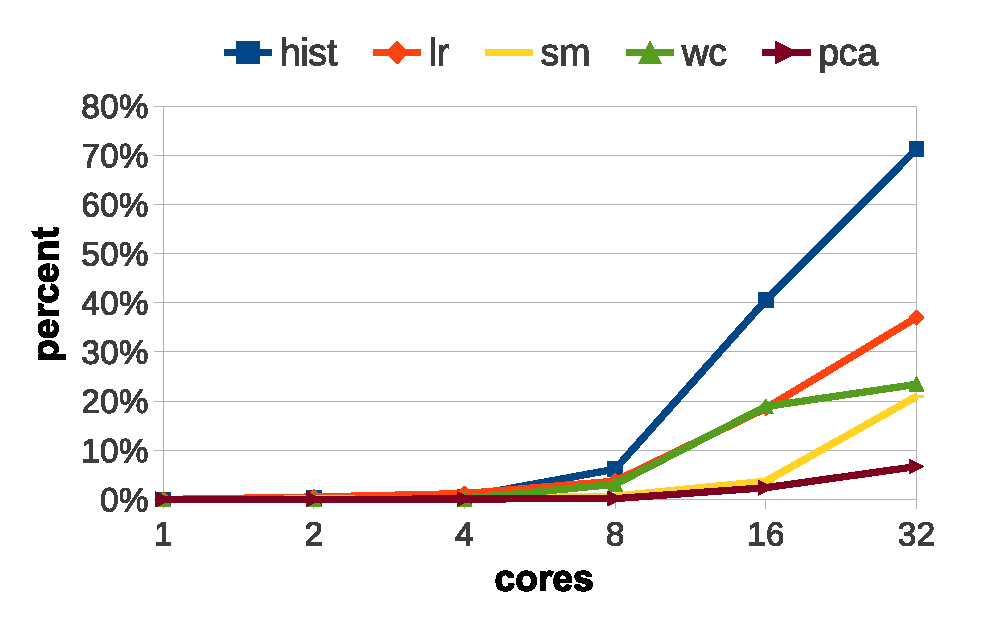
\includegraphics[width=0.45\textwidth]{eps/phoenix_spinlock.eps}
%	\caption{Phoenix ticket\_spin\_lock percent}
%	\label{fig:phoenix:spinlock}
%\end{figure}

Phoenix utilizes shared-memory multiple threads (i.e., Pthread) to implement parallelism, where all threads of an application share a single address space.
In most widely used operating systems, such as Linux, an address space consists principally of a set of memory mapping regions.
Linux use a red-back tree to store these regions. 
The red-back enables the operating system to find a particular region quickly when a process has have thousands of memory regions \cite{linux}.

%store the memory regions because applications often have thousands of memory regions 

%and a tree enables the operating system to find the region
%containing a particular virtual address quickly
%
%One reason why Linux uses this single semaphore on the address space is that it needs a red-black tree to guarantee $O$(log$n$) lookup time when a process has many mmap memory regions \cite{linux}.

The \codet{mmap} operation creates memory mapping regions and adds them to the region red-back tree. 
%munmap removes regions from the tree and invalidates entries in the hardware page table structures. 
Page faults look up the faulting virtual address in the red-back tree check whether the virtual address is mapped.
To ensure correct behavior when several threads perform \codet{mmap} and page faults concurrently, Linux use a single read/write semaphore per process (known as \codet{mmap\_sem}).
To execute the \codet{mmap} operations, threads first need to acquire the semaphore in write mode, while permitting page faults and the other \codet{mmap} operations.
Page faults, which acquire the semaphore in read mode, can proceed with each other in parallel. 


In Phoenix, benchmarks utilize the mmap() system call to read in input data. 
Once the user passes the pointer of the mmap() region to runtime as an argument, multiple map threads will concurrently cause page faults in the input data when they invoke map functions.
%All of these page faults need to access the unique mmap\_sem semaphore, which is local to a process address space. 
Although mmap() system call in applications will not cause contention,
there are mmap operations in memory allocator for heap manage.
By using \codet{mmap\_sem}, Linux can serialize mmap operations and page faults, while limiting the scalability of multithread applications.
The contention is intense when there are large amounts of threads,
which will lead to the parallel scalability degradation on the benchmarks.
%As a result, multiple threads concurrently pagefaults will casue contention to the single semaphore.
 
%The semaphore is a sleep lock and may run into convoying problems,
%where waiting threads may get stuck at the end of the wait queue for a long time \cite{Andi2009lmulticore}.




\subsection{Optimizing Opportunities of Phoenix }
First, in cluster environment, network bandwidth is the key factor for performance since the map and reduce workers, executed in different machines usually, communicate by the network.
However, when processing MapReduce applications in multicore environment, the data structures shared by multiple threads, instead of the network, are the major performance bottlenecks.
By using  a share-memory threads model, Pthreads, multiple threads in Phoenix need to share the process's address space\cite{linux}.
In fact, there is a single lock for per shared address space inside the operating system’s virtual memory system. 
As a result, multithreaded applications on many-core processors will naturally suffer from serious contended locks.
This phenomenon will be common for parallel programming with shared-memory multithreading \cite{clements2013radixvm}.

%多核环境下,限制mapreduce性能的关键因素是多线程共享的数据结构。phoenix是基于共享内存的Pthreads多线程编写的,其中每个线程没有自己独立的地址空间,它们需要共享进程的地址空间,在linux中,每个进程地址空间有一个锁对应,当多个线程需要共享时,便会对这个lock竞争,这种现象对于基于共享内存的多线程并行编程非常普片。

%which would be common for parallel programming with shared-memory multithreading.
Second, there is a strict barrier between the Map and Reduce phase, requiring that the workers in Reduce phase can be started only when all workers in Map phase has been finished, 
%therefore this barrier limits parallel computing.
which limits parallel computing.
And the execution time of the Map phase is subjected to the slowest map worker, which means that if one of the map workers is slow, then the runtime will need more time.
%\bluet{If one of a map worker is slow, then the runtime of MapReduce will be need more time.}  
What's more, it is worth menthion that the user-defined map functions are usually computation-intensive while the Reduce phase is memory-intensive. Thus, the serialization of the Map and Reduce phase is bad for the utilization of system hardware resource.
%barrier不利于资源的利用
%由于map和reduce阶段之间存在一个barrier,只有当map worker全部结束之后,reduce才开始工作,这种严格的barrier不利于并发,并且,如果其中一个map worker花费太多时间,会让真个的运行时间变长,另一方面,由于map 是computition-intensive,而reduce是memory-intensive,Map和Reduce阶段的串序执行,不利于硬件资源的利用。

%In conclusion, Phoenix can not achieve desired scalability with increasing core count because of the strict barrier and contented lock.
%\redt{To achieve scalable performance while retaining the simplicity of the runtime-based approach, it becomes crucial to address these issues.}
To aviod the aforementioned issues, a novel MapReduce model, \myds,  is proposed in this paper,
%employ/exploit/utilize/use
which exploits the producer-consumer model to break barrier and adopts a new thread program model to reduce lock contending.
The implementation details of \myds are presented in Section \label{sec:design} and Section \label{sec:runtime}, respectively.  






%为了避免上述提到的问题,我们希望我们新设计的系统,拥有以下两个特性(1)break barrier (2),提升scalability



\section{Design of thread model}
%这一部分,我们首先分析Phoenix较差scalability的根本原因,然后针对Phoenix scalability存在的challenge,我们提出可行的解决方案,即构造一种具有较好scalability的thread model。具体的实验部分将在section6做详细的解释
{\color{red}In this section, we will search the main factor of Phoenix's bad scalability.
Then we present a new thread model, which has good scalability.
}

\subsection{Scalability of Phoenix}
In Phoenix, programs are often written to start as many threads as the system has cores,
As indicated by figure\ref{fig:phoenix:speedup}, 
when the system is larger than their scalability limit 
adding more threads might actually scale negatively.
The time of completing a workload for one core increases 
when there are more cores in the system. 
The trend of this curve suggests that
the parallel scalability of Phoenix is poor.

In order to understand the scalability behavior, 
Perf\cite{} is exploited to collect execution time information
on the function basis. 
Figure\ref{fig:phoenix:spinlock} shows the percent of \_\_ticket\_spin\_lock of each benchmark.
Histgram on 16cores and 32 cores
show that \_\_ticket\_spin\_lock is one function 
which have largest execution time with 71.25\% and 40.15\% respectively. 
Experimental results show that Phoenix suffer from serious lock contention
when the core count exceeds 8.
\bluet{From Seciton2.2, Phoenix takes two strategies to avoid lock contention.
Why the benchmarks suffer from serious lock contention?
It caused by linux kernel.}
\begin{figure}[!h!t]  
    \centering
    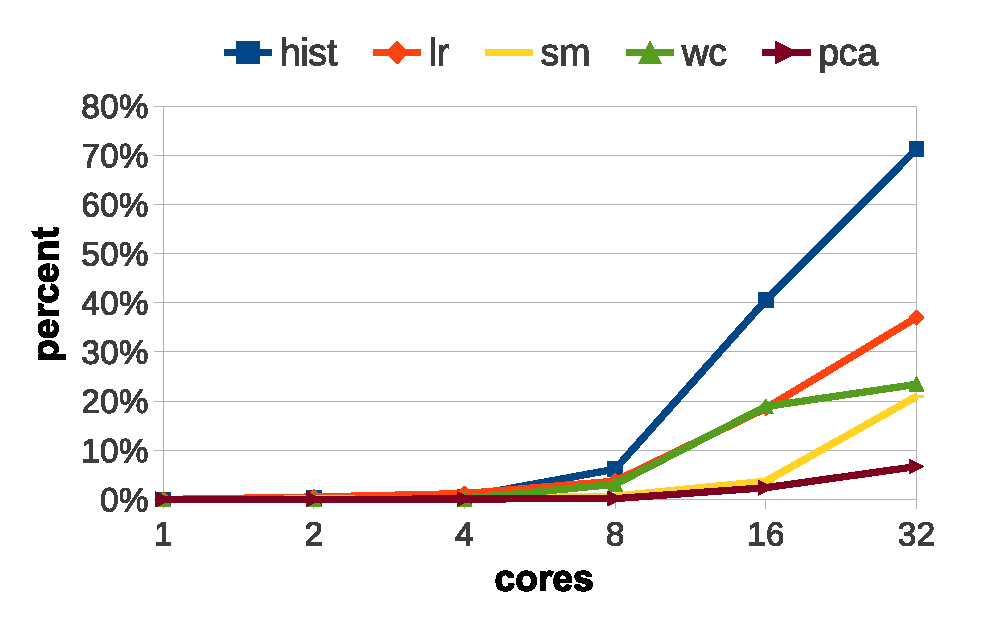
\includegraphics[width=0.35\textwidth]{eps/phoenix_spinlock.eps}
    \caption{Phoenix spinlock percent}
    \label{fig:phoenix:spinlock}
\end{figure}


%Phoenix采取了划分和barrier的方式,以避免多个线程对共享区域的的竞争,为什么还会存在如此高的spinlock呢,
There is a sense in the community that traditional kernel
designs won’t scale well on multicore processors: that
applications will spend an increasing fraction of their time
in the kernel as the number of cores increases.
To understand the Linux scalability
behavior, we analyze the related implementation of Linux
kernel and exploit performance tools to identify scalability
bottlenecks.

Data structure private locks can be a problem 
if the data structure is shared by multiple threads. 
A standard example here are the mm\_sem read-write semaphore 
that protects the list of mappings in a process and 
the pagetable\_lock that protects the pagetable state of a process. 
These locks are local to a process’ address space. 
\bluet{In Phoenix, there is one master process,
and map worker or reduce worker are threads belong to the master process}. 
However when the process is using multiple threads 
then these threads will be able to access the address space in parallel,
which can cause contention on these locks.
%Call-graph information
%and source code analysis show that the two functions are
%called when adding a virtual memory address range into the
%process address space or deleting a virtual memory address range. 
Call-graph information and source code analysis show that 
\_\_ticket\_spin\_lock is caused by pagefault.
When a large multi-threaded computing job 
that causes a lot of parallel page-faults, 
these page-faults will all run into contention on the mm\_sem semaphores.
Semaphores are sleeping locks 
and may run into convoying problems 
where waiting threads may 
get stuck at the end of the wait queue for a long time.\cite{Andi2009lmulticore}
Thus, spin lock 
contention degrades the parallel scalability performance of 
the benchmark. 


%Unfortunately these programs are often written to start as many threads as the system has CPUs, 
%but when the system is larger than their scalability limit adding more threads might actually scale negatively.
%The first measure is to limit them to the maximum number of threads that they can successfully scale to.
%This of course leaves some of the CPUs idle. 

%Performance data reveal that two functions vma link() and
%unlink file vma() have the largest execution time (46.02%
%and 49.97\%) and lock contention. Call-graph information
%and source code analysis show that the two functions are
%called when adding a virtual memory address range into the
%process address space or deleting a virtual memory address range. 
%When multiple slave processes call mmap() or unmap() concurrently, the 
%memory mapped file address range should be added into or 
%deleted from each slave process address space. However, 
%the same spin lock protecting the memory mapped file 
%address range should be held or released. Thus, spin lock 
%contention degrades the parallel scalability performance of 
%the benchmark. 



%The difference between processes and threads under Linux 2.4 is that threads share more parts of their state (address space, file handles etc) than processes, 

\subsection{Separate Address Space}
%这一部分,我们不提生产消费模型,
%为什么要进行地址空间隔离,通过新的线程模型,我们实现了地址空间隔离,隔离之后有什么好处?相比Phoenix,我们这种新的模型会不会带来开销。
One reason that widely used operating systems 
use a lock on the address space is 
that they use complex index data structures to guarantee O(log n)
lookup time when a process has many mapped memory
regions. Linux uses a red-black tree for the regions\cite{linux}. 
Because the data structures require rebalancing 
when a memory region is inserted, 
they protect the entire data structure with a single lock.
The lock is local to a process address space.
when the process is using multiple threads 
then these threads will be able to access
the address space in parallel, 
which can cause contention on the lock.
%随着核数的增多,这种问题会更加突出,最好导致较差的scalability
\bluet{As the increasing of cores number, 
the scalability will be bad.
}

Our goal is to make page faults scale to 
large numbers of cores.
This requires addressing a basic problem,
How allow page faults to run concurrently to eliminate on the per-process read/write lock.
This is difficult because of complicates sharing.

To achieve our goal, this paper persents a new concurrent address space design that eliminates the above sources of contention by applying a new program model and by introducing channel, a way to share data between threads.
We aim at providing an race-free programming abstraction 
to support scalable MapReduce.
%We aim at providing an easy-to-use programming abstraction 
%to support scalable MapReduce.
\bluet{
With this target, we propose a new thread programming model \myth(Scalable thread).
%We propose a new thread programming model to support efficient pipeline parallelism.
%新的线程模型与传统的Pthread模型的主要不同在于:(1)每个线程拥有自己独立的地址空间,这样可以避免多个线程对mm\_struct结构的竞争。(2)线程之间有一个共享的通道,同于线程数据的共享。
\myth is C library-based and 
thread in \myth run in separate memory spaces.
Threads in Pthreads share the address space of the process that created it, 
while threads in \myth have their own address space,
meaning each thread has a mm\_struct.
Therefore, thread no need contend with others thread for lock.
On the other hand,
Threads based on share space can directly communicate with other threads of its process; 
While \myth must use interprocess communication to communicate with the other threads.
We provoide a share channel for threads to communicate.
The initial state of isolated memory in a thread is inherited from
its parent thread when it is started. 
Currently, there is no shared heap among threads, 
but private heap for each thread.
On the other hand, comparing to thread, it is bad for sharing data between threads.
To solute the problem, \myth provide interface of channnel to 
create, send, receive opration.
}
\label{sec:pm:thread}
\begin{figure}[htpb]
\input chanapi.tex
\caption{Main functions of \myds thread API.}
\label{fig:api:thread}
\end{figure}



%mapreduce中是如何使用这个简易的模型进行编程和实现的,这个模型潜在的开销是什么
Figure\ref{fig:api:thread} lists main function of managing threads and channels in \myth.
Initialize in \myds, the master threads invoke 
\codet{thread\_alloc} to create map workers and reduce workers
, and invoke \codet{chan\_alloc} to alloc channels for them.
In \myds map and reduce are implemented using a producer-consumer model.
The map threads and reduce threads are
the producers and consumers, respectively
(Section 4).

Map worker, producing key-value, send message(calling \codet{chan\_setprod}),
and reduce worker as a consumer to receive message(calling \codet{chan\_recv}).
After creating channels and setting up send-receive relationship,
both map and reduce workers start work by invoking \codet{thread\_start}.
When the local buffer is full, 
Map worker invoke \codet{chan\_send} to send
the key-value to coresponded channel.
Then Reduce worker invoke \codet{chan\_recv} to receive
the key-value from the channel. 
Though, using \myth can effectively decrease the overhead of contention,
it also take some extra overhead comparing to Phoneix. 
The extra overhead focus on initialization(section 5). 







\subsection{Design of the Channel}

%channel的底层实现,以及它无限制的映射机制,想说明的问题是:不需要等待,且没有过多的malloc和free操作带来的开销。
Once the channel relationships are set up, 
map workers can invoke \codet{chan\_send} to send messages to channel,
and reduce workers can receive from the channel by \codet{chan\_recv}.
%MPI中的channel是不是要等待,是不是预先分配一块固定的大小。
In order to avoid map waiting when the channel buffer is full,
we design an unbounded size of communication buffer.
Therefore, a sender can send any number of messages without blocking or waiting.
Unboundedness goal is the key to achieve high throughput.
%这个特性的好处

In order to reach a unbounded buffer,
We design an extend machanism 
which allows remap channel’s buffer to a new page frames.
To record and trace generations of page frames among the sharing parties, 
a special anchor extension page is introduced and shared between producer thread and consumers consumer.
Initially a sequence of pages in channel buffer 
are mapped to a \codet{anchor} page table (Anchor in Figure
\ref{fig:spmckern:extend}), 
in which each page has a corresponding page table entry (PTE).
Upon a producer page fault, the fault handler will allocate a real page frame and update the faulting page with a
writable producer mapping so that the producer can write the
page afterwards.
When a thread want to send without waiting, 
it can call extend primitive to remap channel buffer to new page frames,
without changing the old page 
that consumers may still require. 
After a consumer receive the old page from the channel, 
it can call extend to find the new page frames sended by the
producer.
The older page frames decrease their reference counts and
are freed automatically when the counts reach zero.


\begin{figure}[!h!t]  
    \centering
    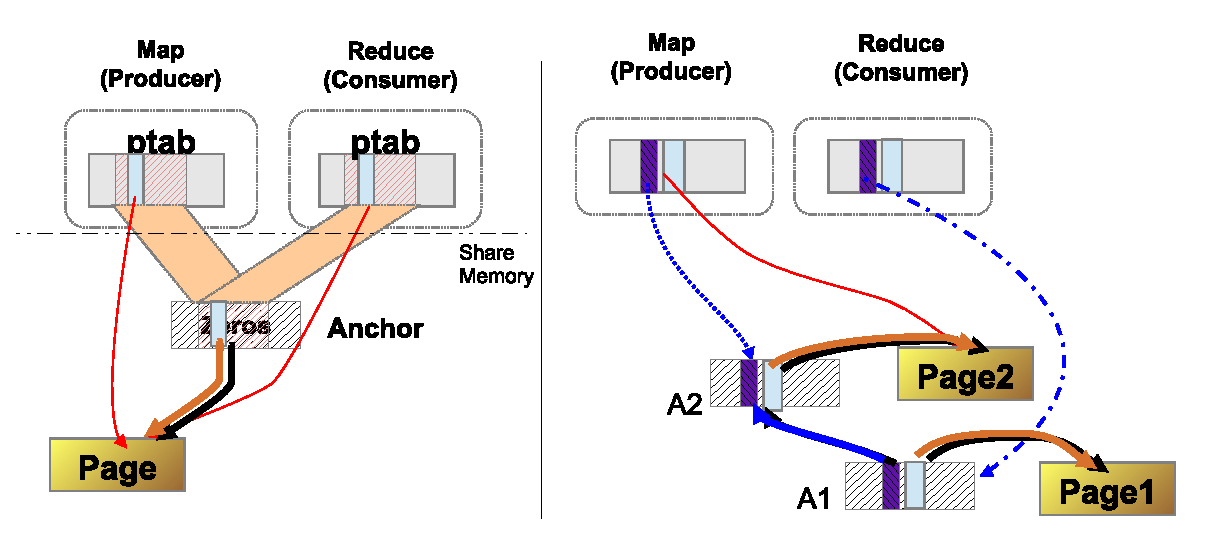
\includegraphics[width=0.5\textwidth]{eps/spmckern_extend.eps}
    \caption{channel extend machanism}
    \label{fig:spmckern:extend}
\end{figure}


%\begin{figure*}
%\centering
% \subfigure[]{
%  \label{fig:spmc:kernext:a}  
%  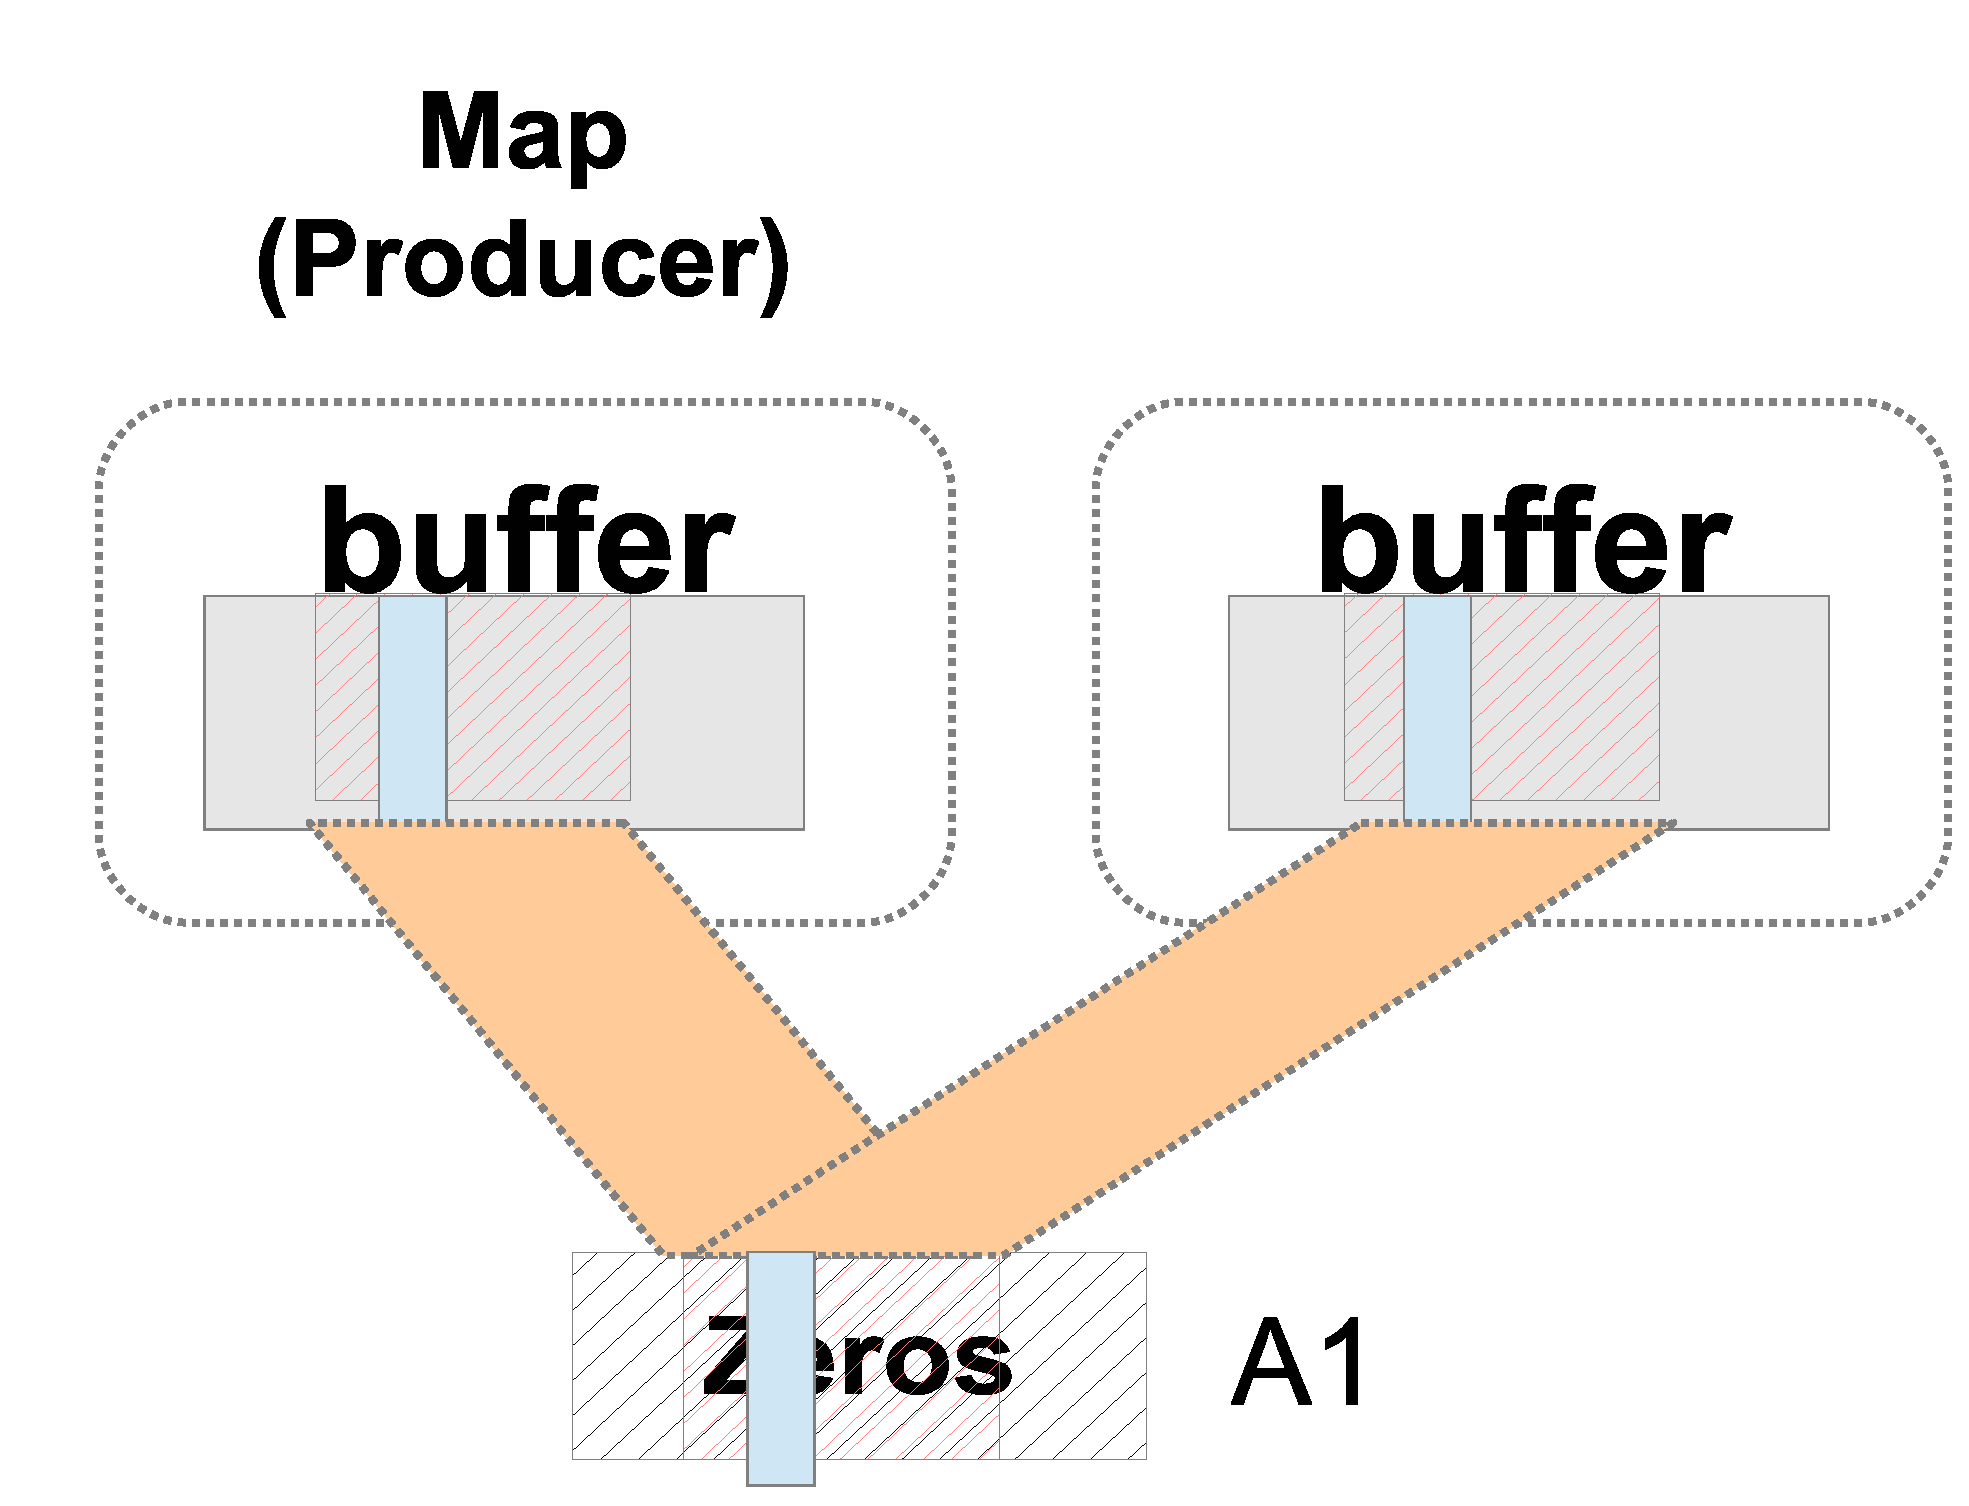
\includegraphics[width=0.23\textwidth]{eps/spmckern-ext0.eps}
% }
% \subfigure[]{
%  \label{fig:spmc:kernext:b}  
%  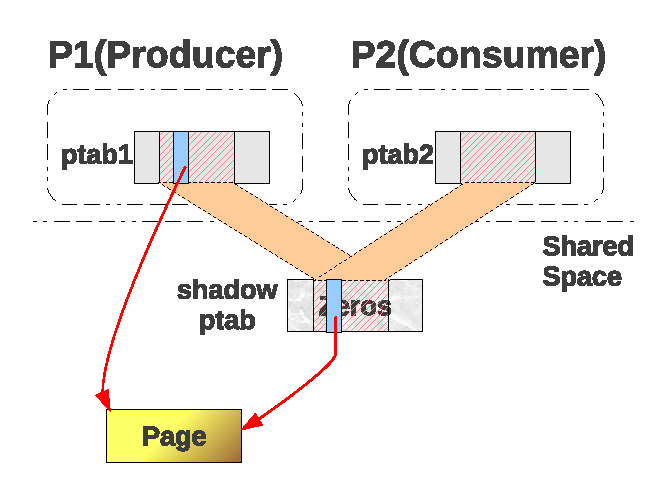
\includegraphics[width=0.23\textwidth]{eps/spmckern-ext2.eps}
% }
% \subfigure[]{
%  \label{fig:spmc:kernext:c}  
%  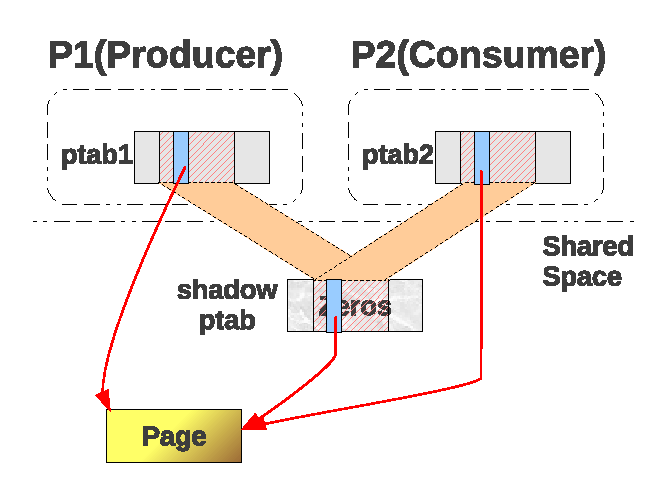
\includegraphics[width=0.23\textwidth]{eps/spmckern-ext3.eps}
% }
% \subfigure[]{
%  \label{fig:spmc:kernext:d}  
%  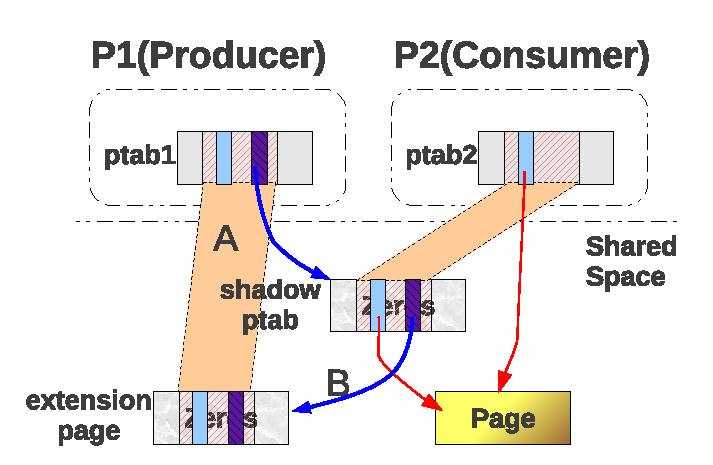
\includegraphics[width=0.23\textwidth]{eps/spmckern-ext4.eps}
% }
%\caption{Mechanism of SPMC virtual memory with lazy page mapping and space extension.}
%\label{fig:dmr:spmc}
%\end{figure*}

%最后,结合mapreduce来说明这种结构的优势在何处













\subsection{SMR的dataflow}
\subsection{流水线并行}
%主要讲述流水线并行的优势,以及各个部件,上层能够看到的,下一章再来详细介绍底层实现上的支持
如上问所述,影响Phoenix性能的关键因素是
barrier的存在,
以及Posix线程库较差的scalability。
DMR基于一种新的Producer-Consumer模型,
打破barrier,且不再使用线程库,
从而提高处理的效率和scalability。
本节阐述新的Producer-Consumer的设计原理,
DMR的流水并行,以及地址空间的隔离。

多核下的MapReduce模型中,
Map阶段产生的key-value,都存放于一个共享的中间结构,
之前的很多研究都显示,
影响多核MapReduce系统性能的关键因素是
对该中间结构的操作效率\cite{mao2010metis}。
\begin{figure}[!h!t]  
    \centering
    \includegraphics[width=0.75\textwidth]{img/phoenix_intermediate.eps}
    \caption{phoenix intermediate is a gobal array}
    \label{phoenix:intermediate}
\end{figure}

Phoenix中间结构是一个全局的二维数组
(如图\ref{phoenix:intermediate}),
为了避免多个map worker和reduce worker对
共享的中间结构竞争,
Phoenix采用两种策略:
\begin{itemize}
  \item 对全局的二维数组进行划分:
  每个map操作每一行,每个reduce操作每一列。
  即map和reduce都拥有自己独立的读写区域。
  可有效避免多个map或多个reduce之间读写同一区域的竞争。
  
  \item 为了避免map和reduce的交织,
  Phoenix在map和reduce之间加入barrier,
  即Map阶段结束后,才能开始Reduce阶段。
  可以避免map和reduce对同一区域的竞争。
\end{itemize}

Map阶段通常会进行大量的计算,
Reduce阶段则是需要大量的内存访问。
如果像Phoenix一样,在Map和Reduce之间加入barrier,
即等到所有的Map阶段结束,才开始reduce计算,
就会存在两个问题:
\begin{itemize}
  \item 不利于CPU的利用率,Map阶段会集中使用CPU,
  而Reduce阶段需要大量的内存访问,
  CPU资源被浪费。
  \item reduce阶段开始时间,由最慢的map worker决定;
  当某个map worker非常慢,便会影响整体的性能
\end{itemize}

DMR设计实现中,首先打破Phoenix的barrier,
不再使用共享的中间结构,DMR中的每个map worker
都拥有属于自己的私有buffer(buffer的设计细节见下一节),
一旦buffer中的key-value达到一定的阈值便发送给相应的reduce worker,
reduce收到key-value后,不等map worker结束便开始reduce工作,
即Map和Reduce阶段并发的粒度变小,
这既能充分利用资源,又能提高计算的速度。

特别地,当我们采用array buffer,
并且在map阶段不开启combiner时,
Map阶段不需要对key-value排序,即无需key的查找和插入,以及memmove等操作。
map worker产生key-value后,只需简单地将其追加到buffer中即可,
这减轻的Map阶段的工作量。key-value的排序工作由Reduce承担,
reduce worker对收到的key-value进行有序插入。
虽然整个过程的工作量并未减少,
但是Reduce的排序工作与Map阶段是并发执行的,
从而整个过程的时间变小,提高运行的效率。

此外,为了防止数据的倾斜,即大量的key-value被发送到一个reduce worker,
在Reduce阶段,我们添加了局部的reduce过程(即combiner),
一旦某个Reduce收到某个key-value的数量超过预先设定的值,
便会触发combiner,从而避免过多的内存分配带来的开销,
防止内存溢出。

DMR中map worker和reduce worker之所以能够进行流水并行执行,
是因为它们基于一个Producer-Consumer model,
在这个model中,每个map worker都拥有一个私有的buffer,
map woker是这个buffer的生产者,reduce是buffer的消费者,
当buffer中的数据达到一个阈值时,
reduce便可以取到buffer中的数据开始工作,
而不需要等到所有map结束。



\subsubsection{produce-consume模型}
%将详细介绍这个producer-consumer模型的所有特点,
如上所述,map worker和reducer worker的流水执行,
需要底层Producer-Consumer模型的支持,
本节将详细描述该模型的设计原理。

通常producer-consumer模型中,
producer和consumer之间有一个queue,
producer向queue中添加任务,
consumer从queue中读取任务。
MRPhi\cite{lu2013mrphi}为了使Map和Reduce并行执行,
便是采用这种Producer-Consumer模型,
具体如图\ref{mrphi:pc-model}所示。
在这个模型中,每个reduce worker对应一个queue,
map worker产生的数据会追加到queue中,
这是一个多对一的produce-consume模型,
\begin{figure}[!h!t]  
    \centering
    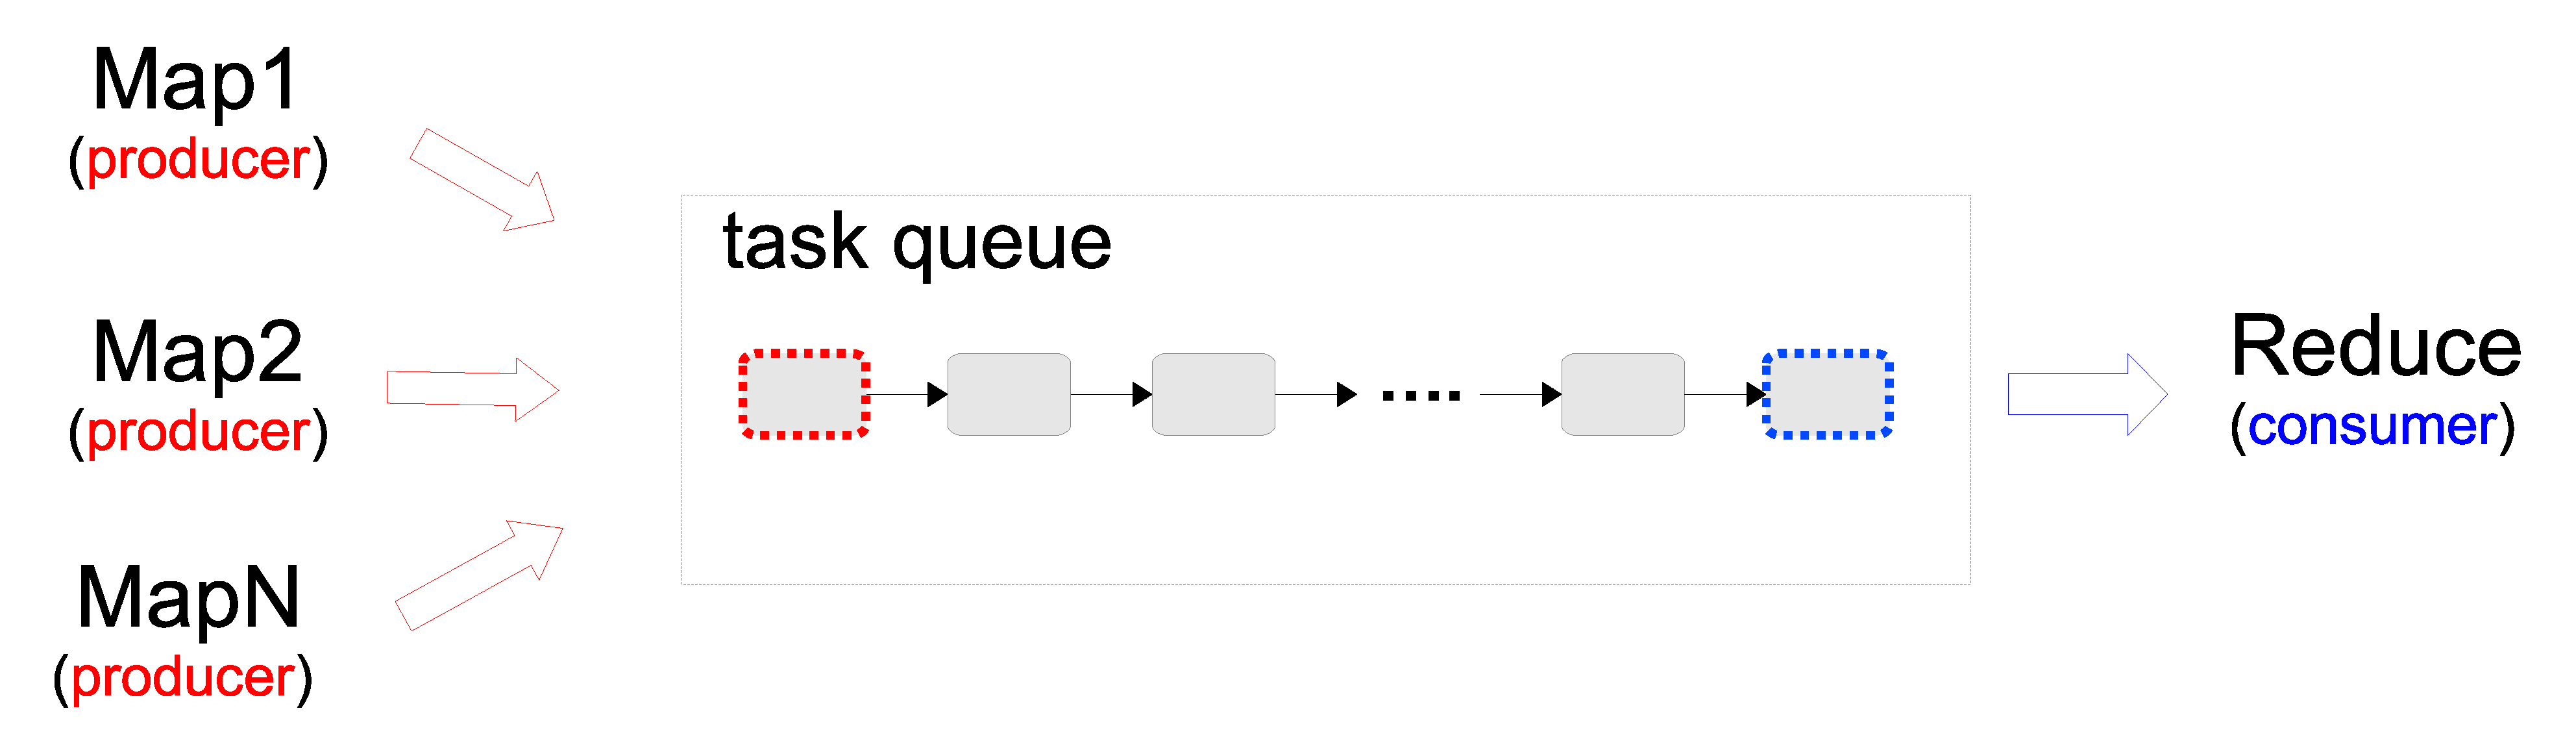
\includegraphics[width=0.5\textwidth]{img/mrphi_pc_model.eps}
    \caption{producer-consumer model in MRPhi}
    \label{mrphi:pc-model}
\end{figure}
虽然MRPhi利用该produce-consume模型实现的Map和Reduce阶段的并发执行,
但是它存在以下两个问题:
\begin{itemize}  
  \item map worker将task插入到queue中之前,需要竞争queue的lock。
  并且线程数越多时,等待lock的开销会越大。
  由于多个map worker同时向task queue中插入任务,
  需要一定的同步机制保证插入的正确性,
  这会造成一定的等待开销。
  \item queue的管理问题,虽然MRPhi\cite{lu2013mrphi}中并没有提到,
  具体的queue是如何管理的,但queue的管理不外乎两种:
  (1)采用固定分配的方式:预先分配一块固定大小的空间,之后重复利用,
  但当queue满,map woker需要停止等待,直到reduce将queue中的数据取走。
  (2)采用动态分配:虽然map worker不需要等待,
  但是会存在大量的动态内存分配和回收的开销。
\end{itemize}
  DMR中使用的producer-consumer模型则不同,
  其中map worker和reduce worker使用一种一对一的隐式queue,
  每个map worker只需将task插入到专属的queue中即可。
  因此,多个map worker不需要竞争queue,从而可有效减少锁的开销。
  
  
\begin{figure}[!h!t]  
    \centering
    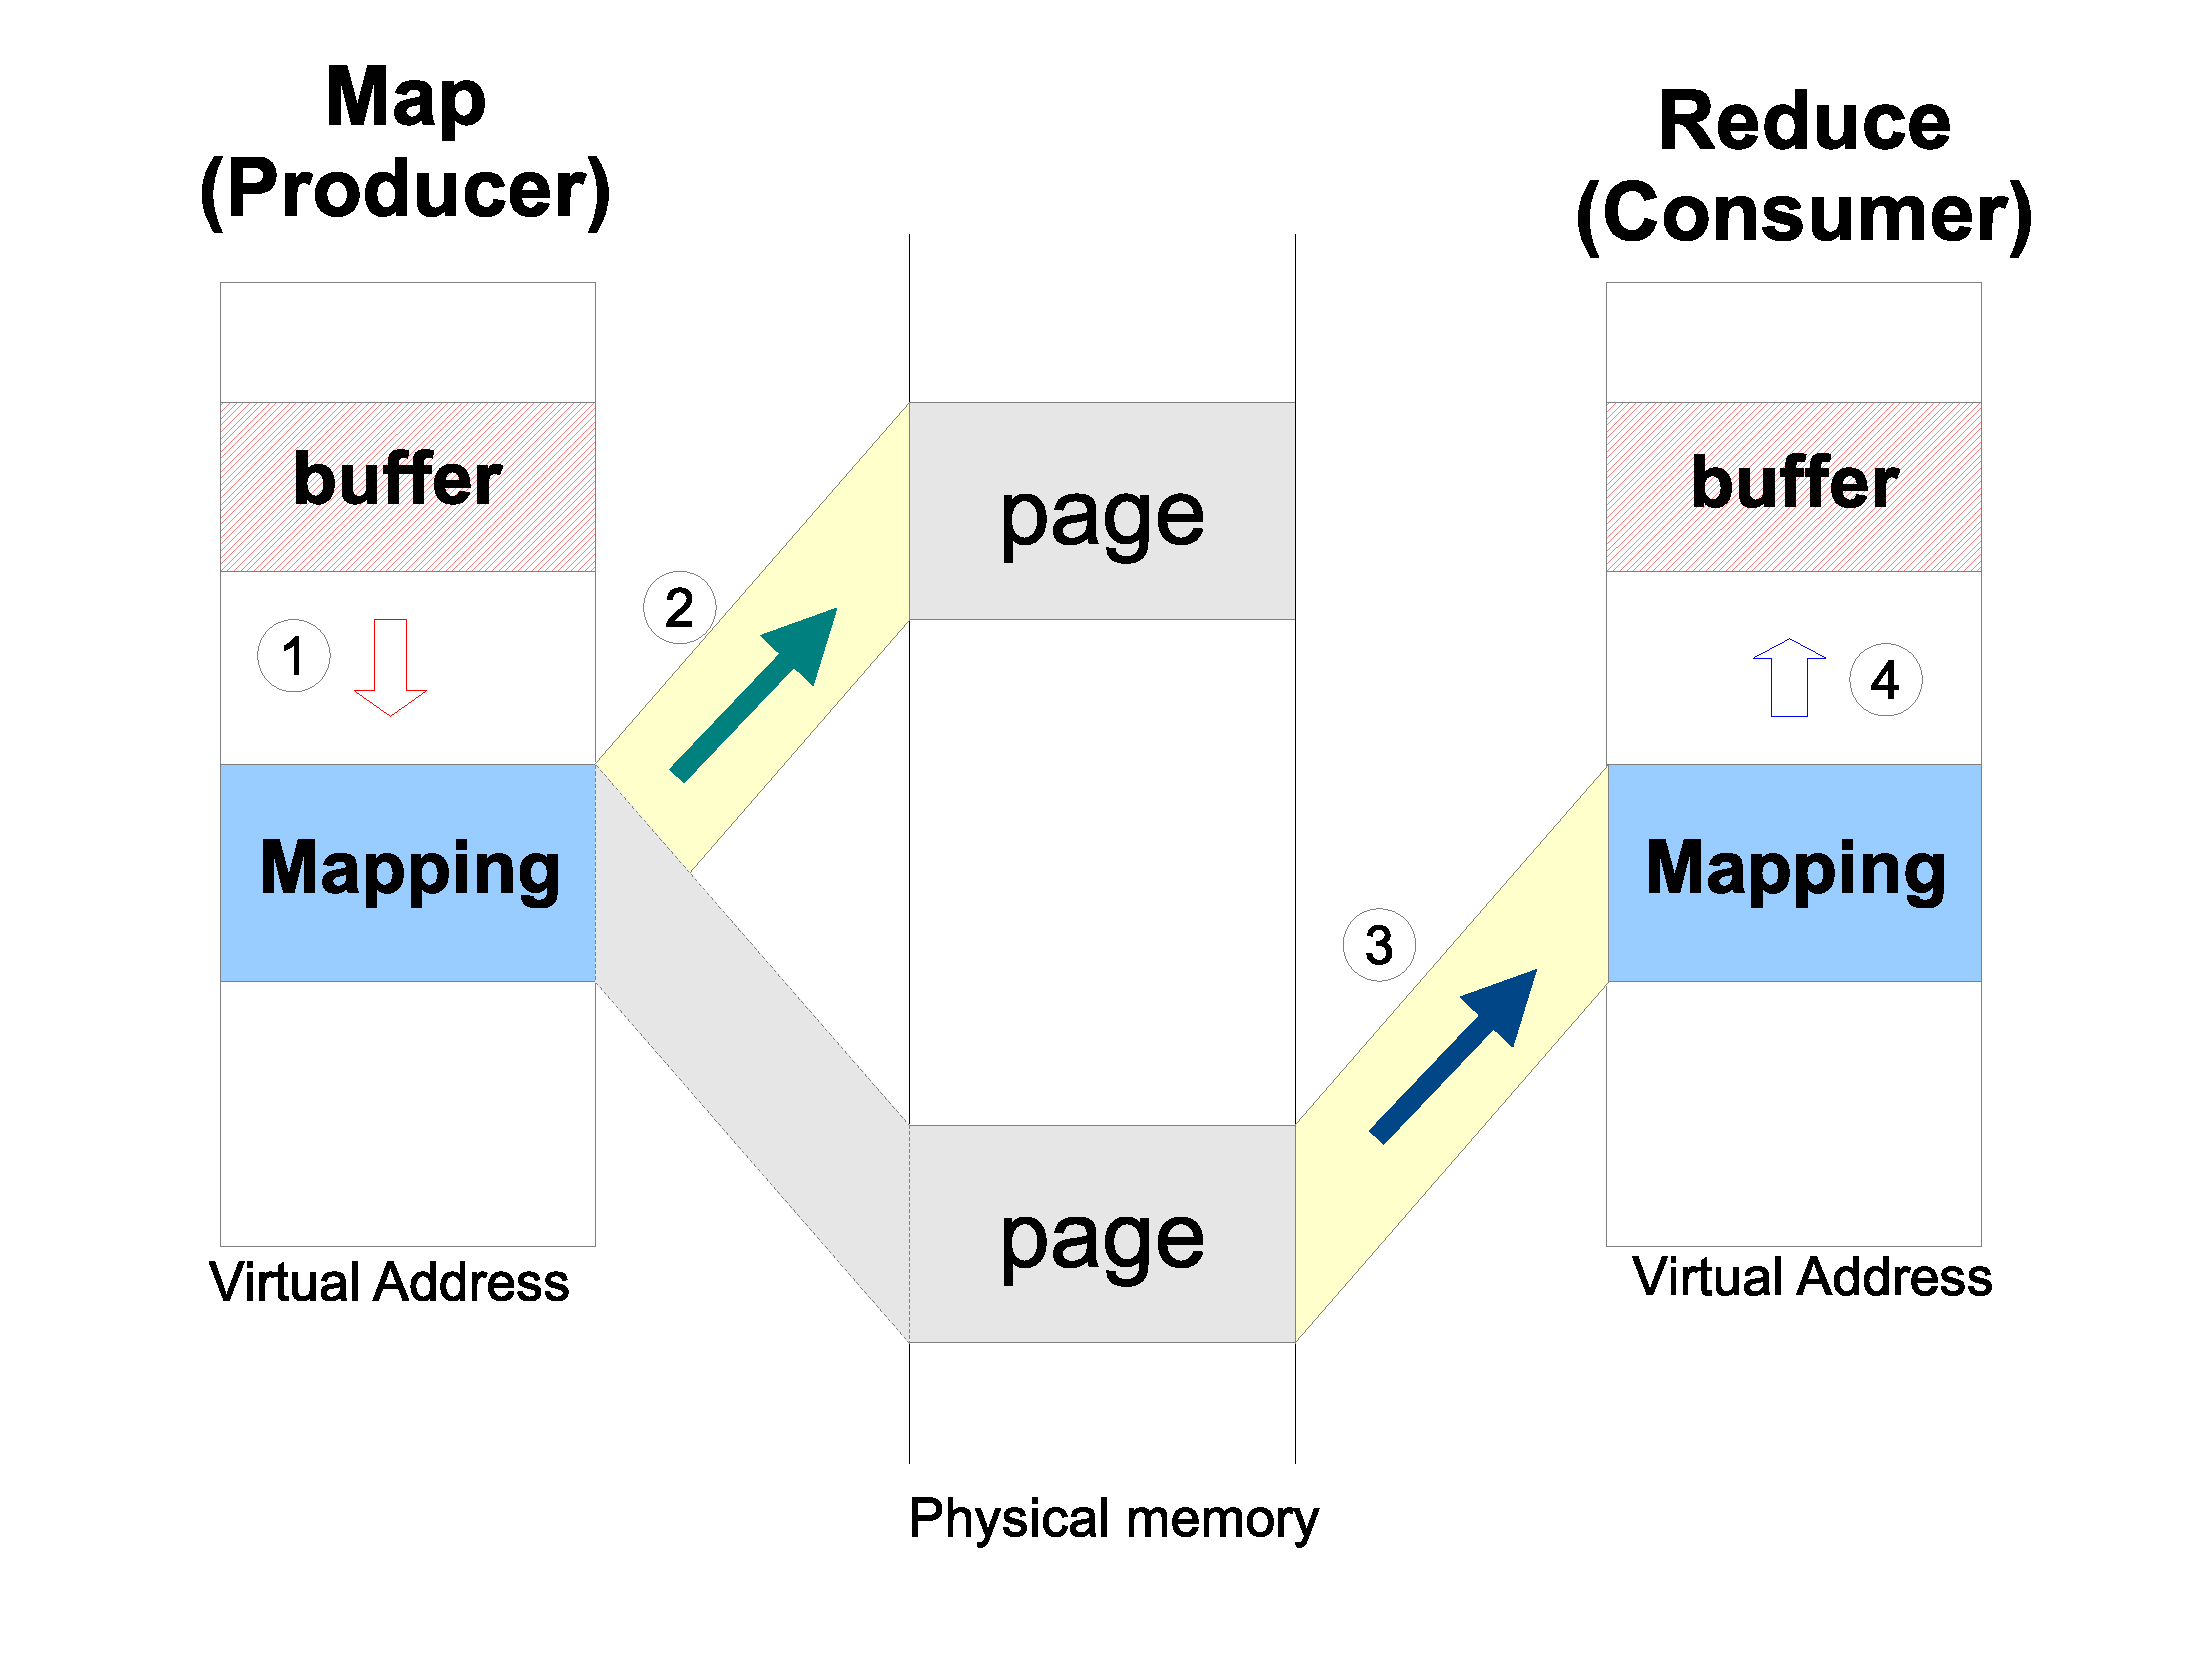
\includegraphics[width=0.5\textwidth]{img/dmr_pc_model.eps}
    \caption{producer-consumer model in DMR}
    \label{dmr:pc-model}
\end{figure}

如图\ref{dmr:pc-model}所示,综上所述,
DMR中producer-consumer模型的关键不同之处有两点:
其一,producer和consumer之间是一对一的隐式queue,
因此producer之间无须竞争,可以避免锁的竞争带来的开销。
其二,producer和consumer之间的隐式queue,
不采用显示的操作,而是采用一种mapping的方式,
即一旦buffer中的数据满,producer便会触发一个send操作,
底层的实现中,会将buffer对应的物理内存加入到隐式queue中,
buffer重新映射到一块新的物理内存,
producer只需将buffer设置为空,
便可继续对buffer进行读写。
这种方式的优点在于其快速高效。

DMR中的具体操作为,map worker向buffer中写入数据,
当buffer满时触发send操作,
之后将buffer标志为空,便可继续向buffer中写数据。
reduce worker以轮循的方式读取各个隐式queue中的数据,
从而,map worker和reduce worker可以并发的进行工作,
且不需要复杂的同步手段。
\input mapbuf

\section{Evaluation}
\label{sec:eval}
This section presents the experimental results for Ostrich on an Intel 32-cores multicore machine. 
We mainly compare the performance of \myds with Phoenix.

We evaluate \myds and Phoenix on a 32-core Intel 4× Xeon E7-4820 system equipped with 128GB of RAM. 
The operating system is Ubuntu 12.04 with kernel 3.2.0 and glibc-2.15.
Benchmarks were built as 64-bit executables with gcc -O3.
We logically disable CPU cores using Linux’s CPU hotplug mechanism, which allows to disable or enable individual CPU cores by writing “0” (or “1”) to a special pseudo file (/sys/devices/system/cpu/cpuN/online), and the total number of threads was matched to the number of CPU cores enabled.
Each workload is executed 10 times. 
To reduce the effect of outliers, the lowest and the highest runtimes for each workload are discarded, and thus each result is the average of the remaining 8 runs.

%\subsection{ Performance Improvements Summary}
%\subsection{Benckmarks}
\subsection{Performance and Scalability}
%描述benchmarks的特点,benchmarks的数据集等
In this subsection, we measured the performance and scalability of \myds, and compare it with Phoenix.  
Since there are many heap objects shared among threads in Phoenix, and it is sensitive to memory allocator.
The memory allocator in glibc (i.e. ptmalloc\cite{gloger1997ptmalloc}), does not scale on multicore system. 
Compared to ptmalloc\cite{gloger1997ptmalloc}, jemalloc provided improved performance and scalability\cite{evans2006jemalloc}. 
Therefore, we evaluate performance and scalability of Phoenix with jemalloc and ptmalloc, respectively.

\subsubsection{Performance}
Based on \myth, we implemented the optimization of Phoenix in Section 4 and measured \myds performance by executing each benchmark, including histogram (\codet{hist}), linear\_regression (\codet{lr}), string\_match (\codet{sm}), wordcount (\codet{wc}), and pca (\codet{pca}). 
\redt{Why use these benchmark?}
Table II describes the workloads and their input datasets. 
\begin{figure}[!h!t]  
	\centering
	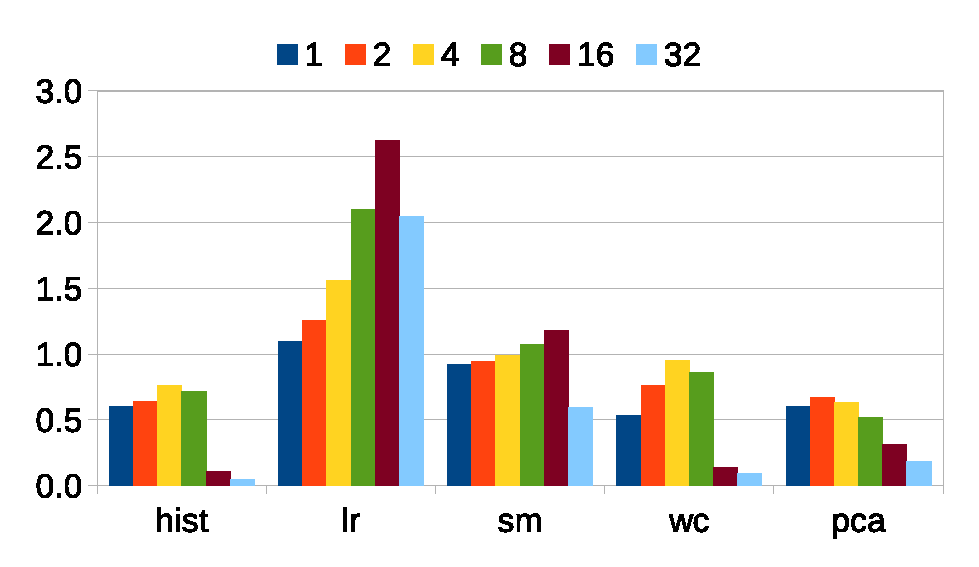
\includegraphics[width=0.45\textwidth]{eps/dmr_time_array.eps}
	\caption{SMR versus Phoenix with ptmalloc}
	\label{fig:smr:time:ptmalloc}
\end{figure}

Figure\ref{fig:smr:time:ptmalloc} measures the relative speedup of \myds over Phoenix-ptmalloc. 
As shown in the Figure \ref{fig:smr:time:ptmalloc}, For \codet{hist}, \codet{wc} and \codet{pca}, the optimized runtime of \myds leads to improvements across all core counts.
For less then 8 cores, the average improvement was \redt{2.0x} and the variation across applications were rather small.
For more then 8 cores, specially with 16 and 32 cores, the improvement were obvious, reaching \redt{10.x} in maximum and \redt{5.0x} on average.
For sm, it has performed as well as Phoenix when the cores number less then 16, while it better than Phoenix when there is more cores.
However, \myds runs worse than Phoenix on \code{lr} (about 0.8x).
\begin{figure}[!h!t]  
	\centering
	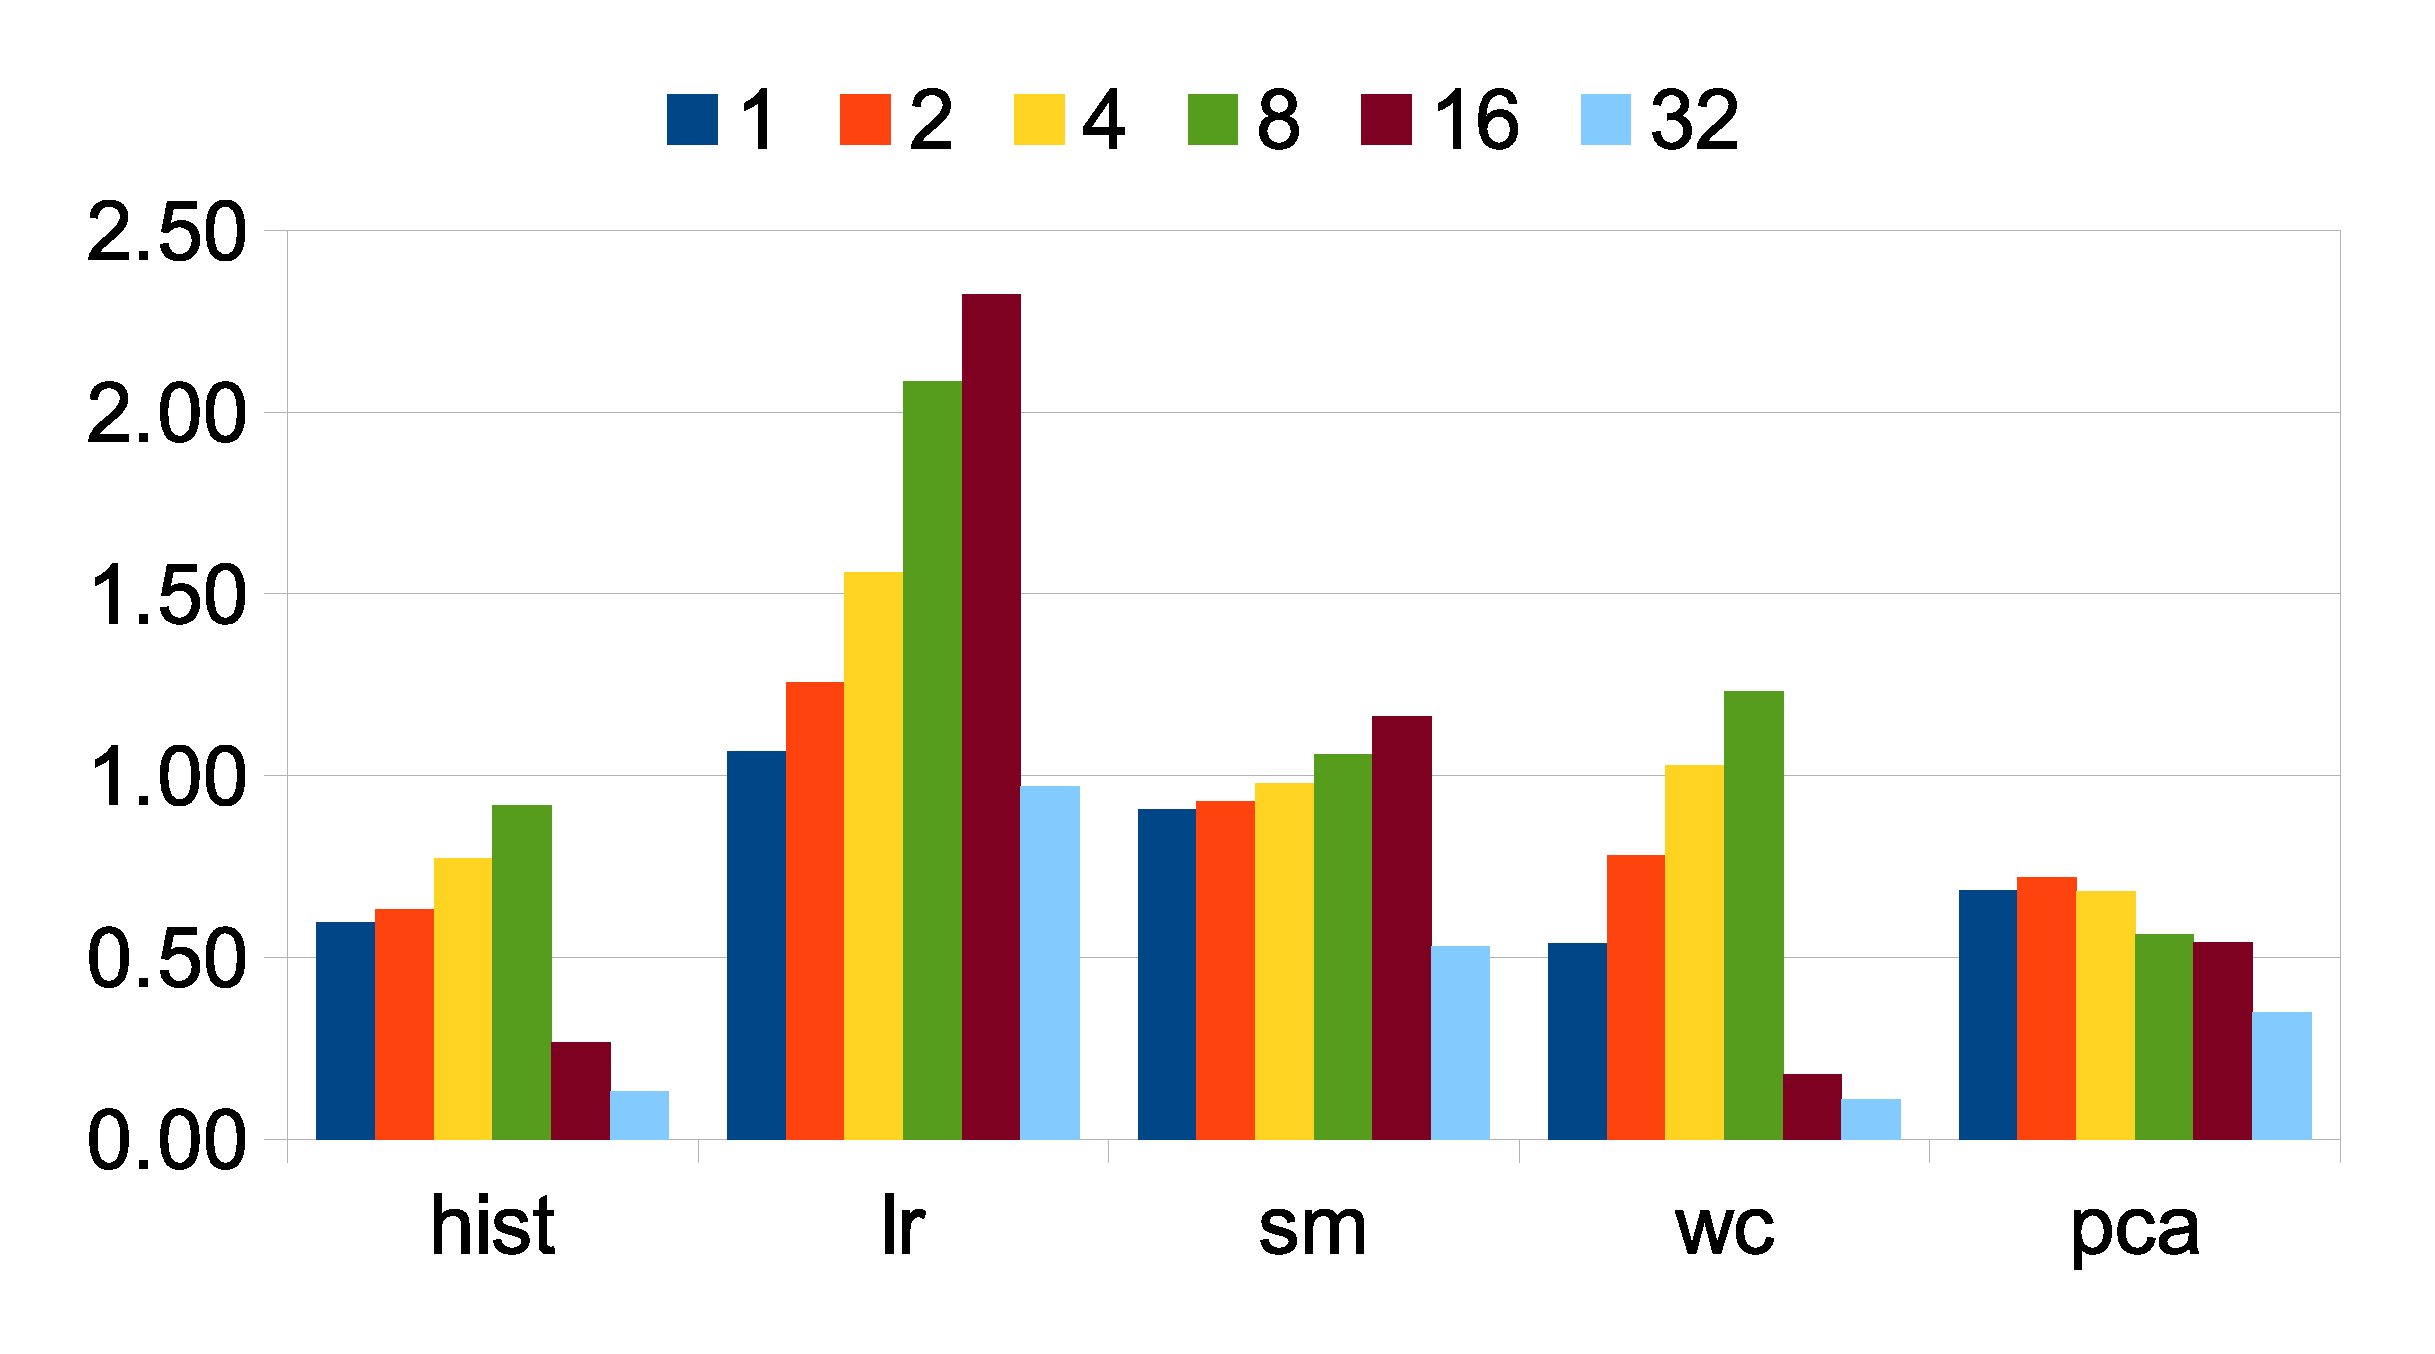
\includegraphics[width=0.45\textwidth]{eps/dmr_time_jemalloc.eps}
	\caption{SMR versus Phoenix with jemalloc}
	\label{fig:smr:time:jemalloc}
\end{figure}

Figure\ref{fig:smr:time:jemalloc} measures the relative speedup of \myds over Phoenix-jemalloc. 
We saw similar tendency when compared with Phoenix-jemalloc in Figure\ref{fig:smr:time:jemalloc}, while Phoenix with jemalloc has a better performacne.
Compared to Phoenix, we significantly increased the performance.
However, workloads, such as \code{lr} and \code{sm}, still did not scale particularly well. 
The reason of worse performance on linear\_regression is that most of time is waste in \myds's initailization.
We will evaluation overhead of initialization time in Section 5.4.
We discuss their bottlenecks in detail in Section 5.4, but in the remainder of this section we first focus on the optimizations that turned out to be successful.
\redt{need to explain why hist, wc, pca has good performance}

%\begin{figure}[htpb]
%	\centering
%	\subfigure[SMR versus Phoenix with ptmalloc]{
%		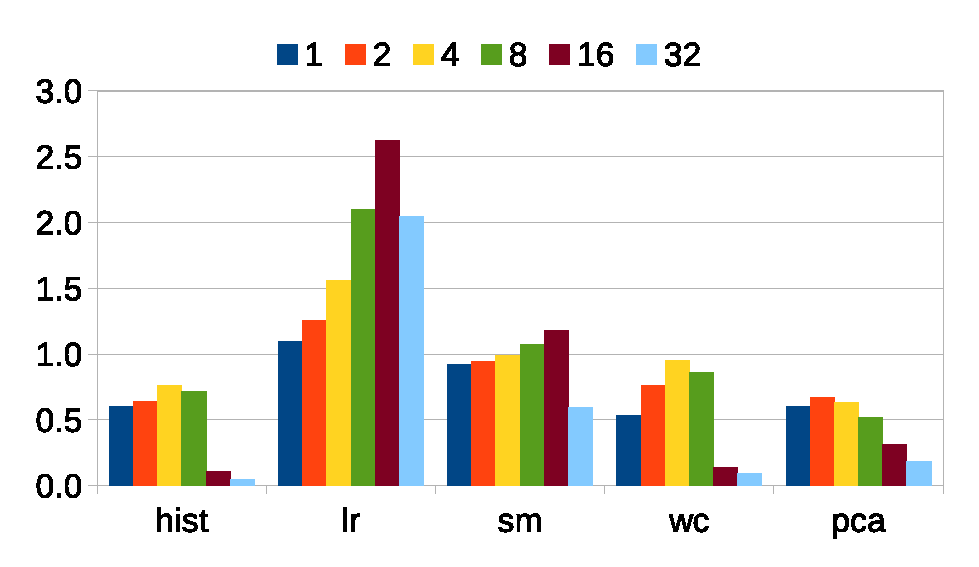
\includegraphics[width=0.45\textwidth]{eps/dmr_time_array.eps}
%		\label{fig:smr:time:ptmalloc}
%	}
%	\subfigure[SMR versus Phoenix with jemalloc]{
%		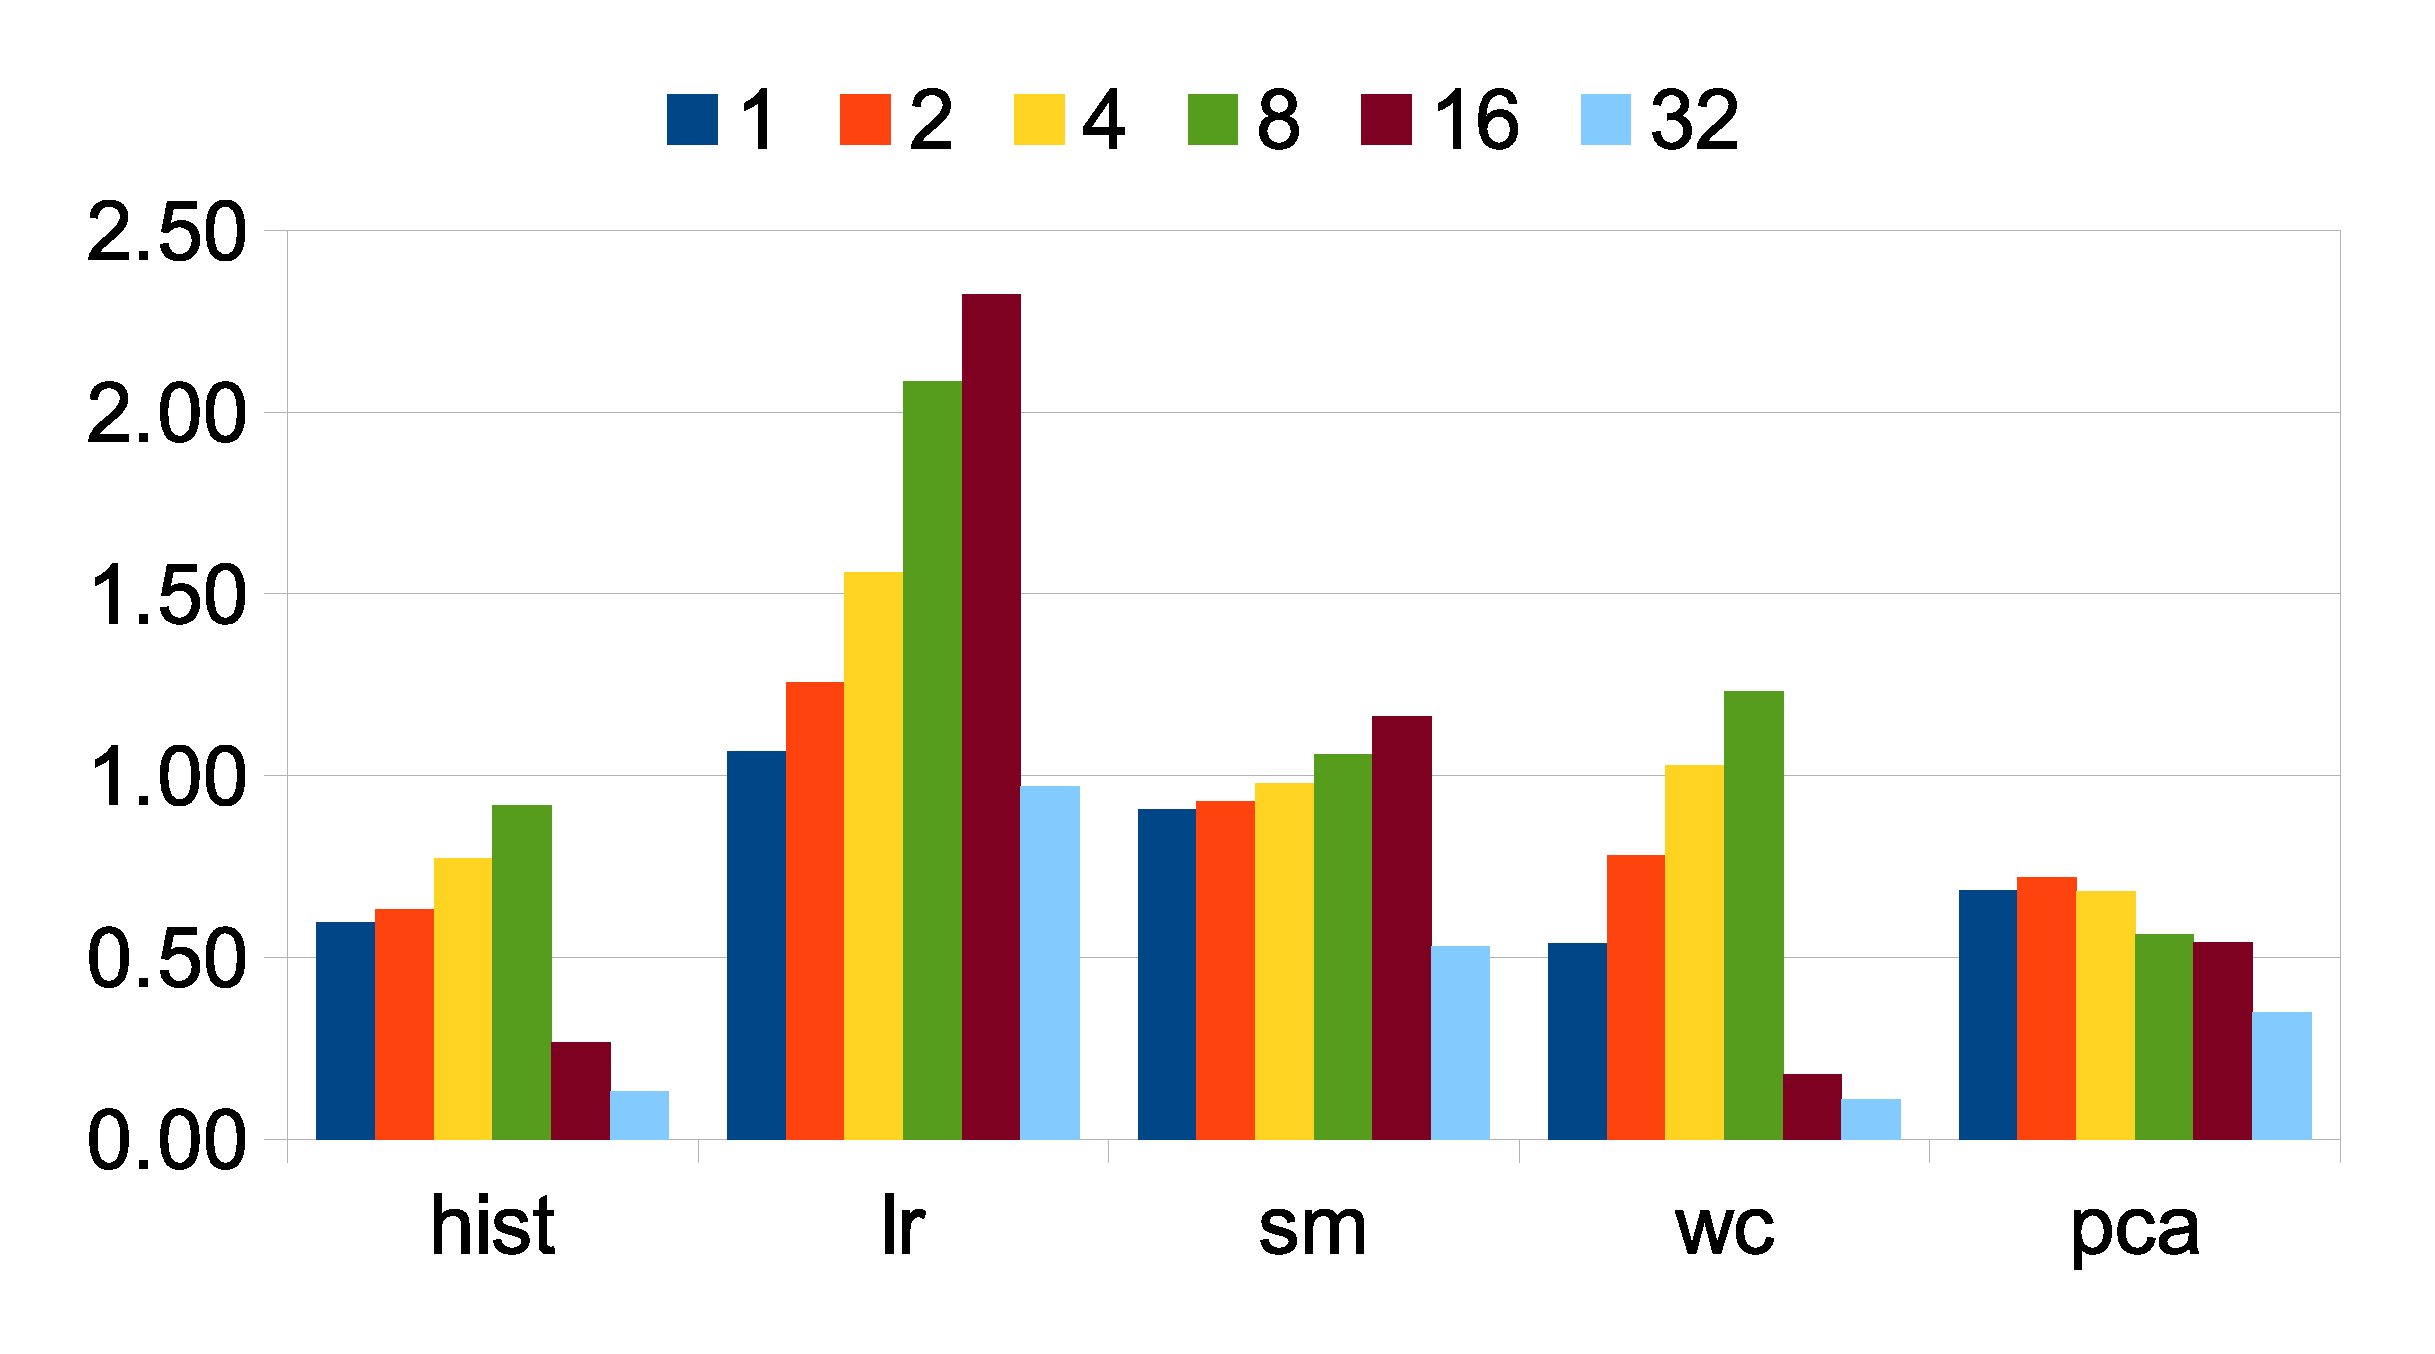
\includegraphics[width=0.45\textwidth]{eps/dmr_time_jemalloc.eps}
%		\label{fig:smr:time:jemalloc}
%	}
%	\caption{Execution time of SMR versus Phoenix}
%	\label{fig:time}
%\end{figure}


%However, nether allocator could successfully scaled up to 32cores.
%
%Figure\ref{fig:dmr:time:ptmalloc} and \ref{fig:dmr:time:jemalloc}
%present the Execution time of \myds versus Phoenix.
%%虽然jemalloc的性能表现要比ptmalloc好,但实验结果都显示
%\myds matches or outperforms Phoenix on 4 out of 5 workloads,
%but runs worse than Phoenix only on linear\_regression.
%For hist, pca and word\_count, 
%\myds outperforms Phoenix betwen xxx and xxx faster.

%从实验的结果可以看出,hist, wc, pca,SMR的性能较好,sm相当,lr中SMR的性能表现较差



%\begin{figure*}[htpb]
%\centering
%  \subfigure[]{
%   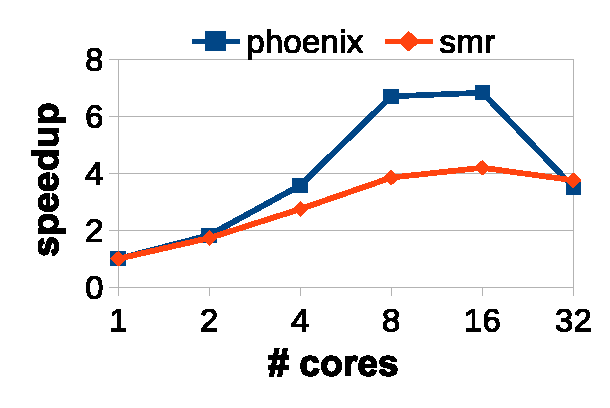
\includegraphics[width=0.15\textwidth]{eps/smr_scala_hist.eps}
%   \label{fig:dmr:time:ptmalloc}
%   }
%  \subfigure[]{
%	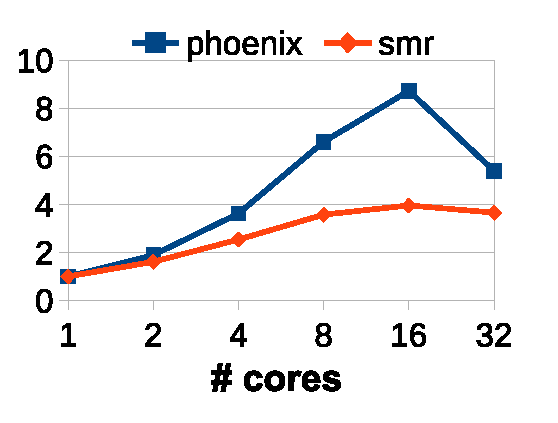
\includegraphics[width=0.15\textwidth]{eps/smr_scala_lr.eps}
%	\label{fig:dmr:time:ptmalloc}
%}
%  \subfigure[]{
%	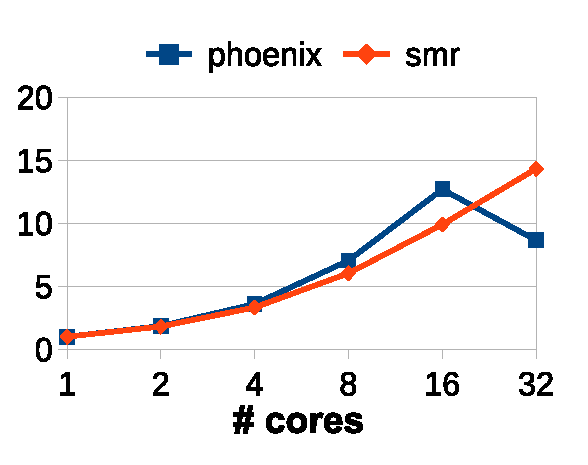
\includegraphics[width=0.15\textwidth]{eps/smr_scala_sm.eps}
%	\label{fig:dmr:time:ptmalloc}
%}
%  \subfigure[]{
%	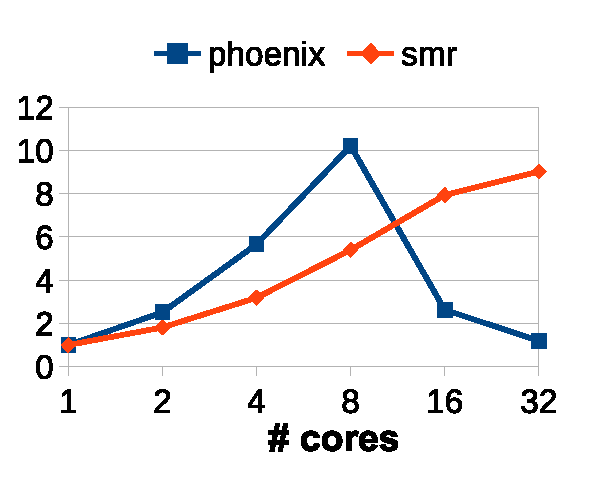
\includegraphics[width=0.15\textwidth]{eps/smr_scala_wc.eps}
%	\label{fig:dmr:time:ptmalloc}
%}
%  \subfigure[]{
%	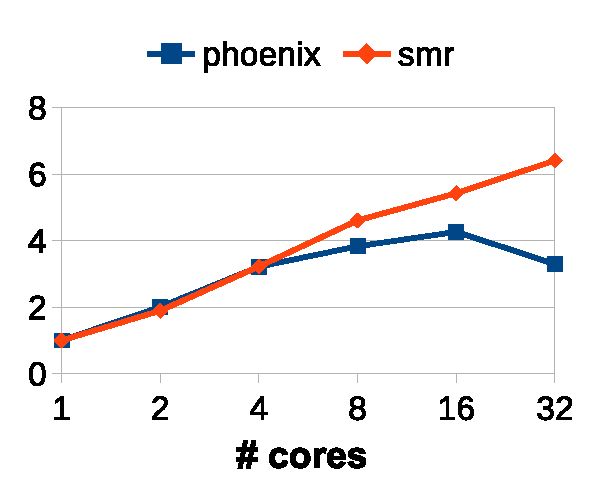
\includegraphics[width=0.15\textwidth]{eps/smr_scala_pca.eps}
%	\label{fig:dmr:time:ptmalloc}
%}
%  \caption{A comparison of the scalability of \myds with that of Phoenix}
%   \label{fig:scalability}
%\end{figure*}

\subsubsection{Scalability}
%Phoenix-jemalloc版本scalability存在的问题
\begin{figure}[!h!t]  
	\centering
	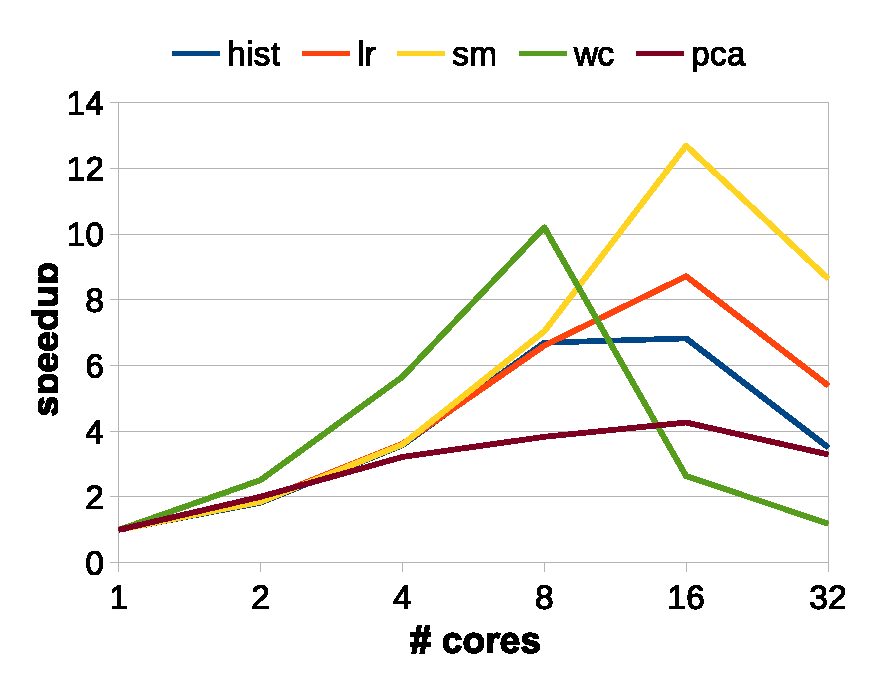
\includegraphics[width=0.45\textwidth]{eps/phoenix_speedup_jemalloc.eps}
	\caption{speedup of Phoenix-jemalloc}
	\label{fig:phoenix:speedup:jemalloc}
\end{figure}

%As shown in this figure \ref{fig:phoenix:speedup}, 
%when using no more than eight cores, the Phoenix scales well on hist ... ;
%when using no more than 16 cores, the Phoenix scales well on sm and le.

%For linear\_regression (lr) and string\_match (sm),  using 16 or more  cores leads to speedup degradation.

Since Phoenix is sensitive to memory allocator, we evaluate its scalability with jemalloc, good scalability allocator.
Figure\ref{fig:phoenix:speedup:jemalloc} shows the speedup of Phoenix with jemalloc.
%\begin{figure}[htpb]
%	\centering
%	\subfigure[speedup of Phoenix-jemalloc]{
%		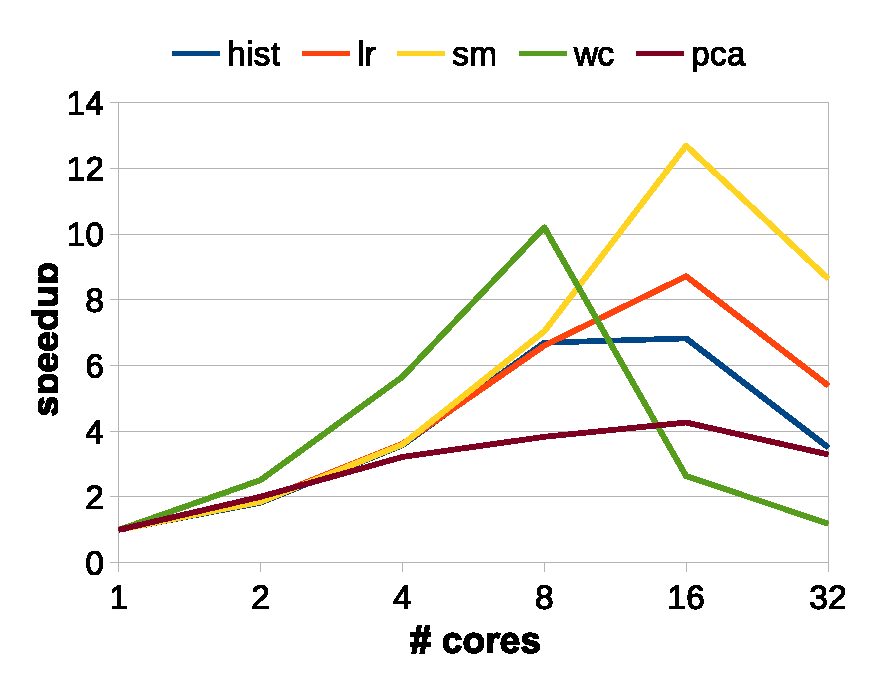
\includegraphics[width=0.45\textwidth]{eps/phoenix_speedup_jemalloc.eps}
%		\label{fig:phoenix:speedup:jemalloc}
%	}
%	\subfigure[\_\_tickect\_spin\_lock execution time percent of Phoenix-jemalloc]{
%		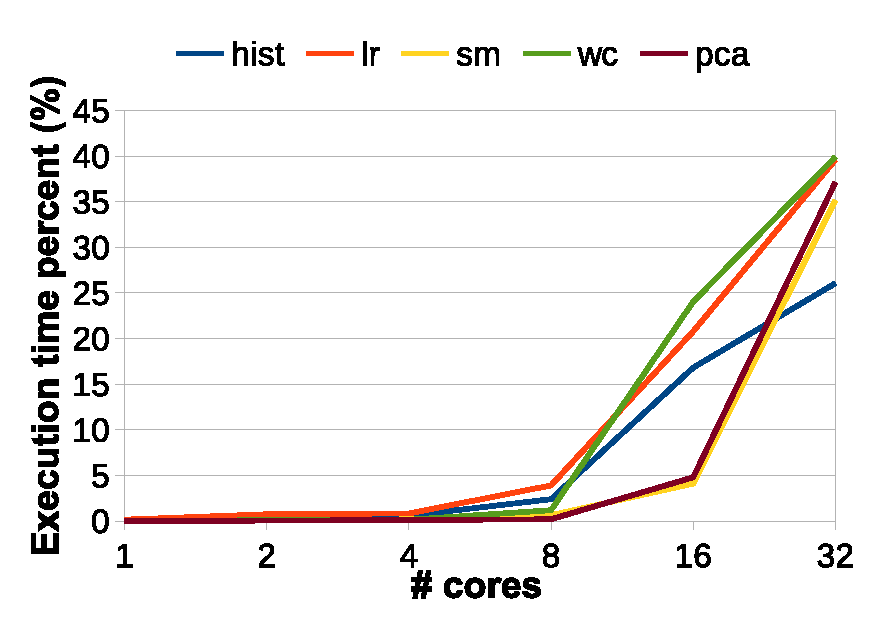
\includegraphics[width=0.45\textwidth]{eps/phoenix_spinlock_jemalloc.eps}
%		\label{fig:phoenix:spinlock:jemalloc}
%	}
%	\caption{scalability of Phoenix-jemalloc}
%	\label{fig:phoenix:scalability}
%\end{figure}
the Phoenix scales well on histgram (hist), wordcount (wc) and pca when the number of core is less than 8.
As for the linear\_regression (lr) and string\_match (sm), 
Phoenix performs well with no more than 16 cores.
However, when core number is more than  8, 
the speedup of Phoenix  on hist,  wc and pca is degraded.
For lr and sm, the speedup is degraded when cores is greater than 16.

%As the number of cores increase (from 1 to 8), the performance of Phoenix increase for all cases, i.e., the execution time decreasing. 
%While For 16 to 32 cores, Phoenix performance keep decreasing with the increase of the number of cores.
\begin{figure}[!h!t]  
	\centering
	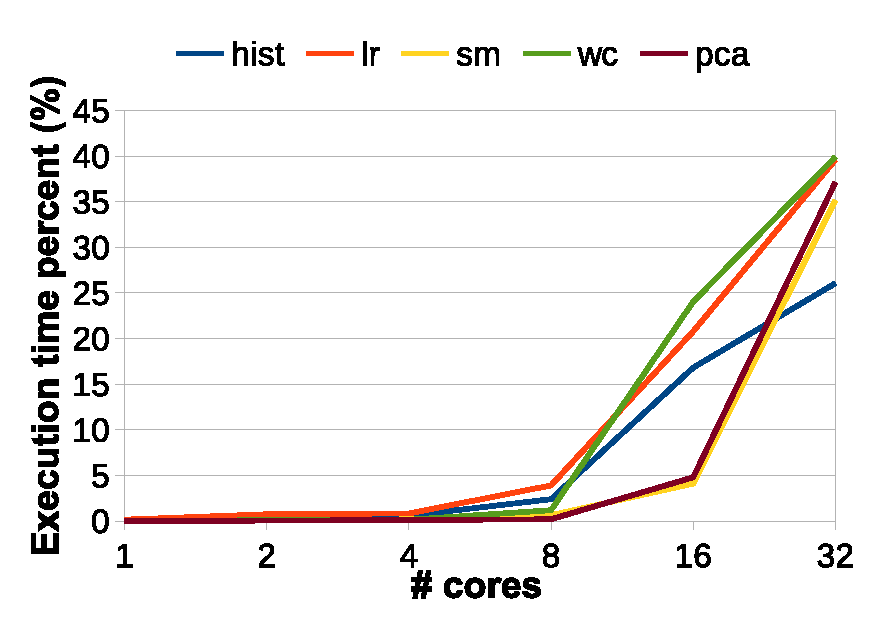
\includegraphics[width=0.45\textwidth]{eps/phoenix_spinlock_jemalloc.eps}
	\caption{speedup of Phoenix-jemalloc}
	\label{fig:phoenix:spinlock:jemalloc}
\end{figure}
At the same time, we collect \_\_ticket\_spin\_lock execution time percent by Linux perf to peek the contention in Linux kernal.
The result shows in Figure\ref{fig:phoenix:spinlock:jemalloc}.
We note serious contending lock takes place when increase the number of cores over 8 and as a result execution time will be drastically increased.
%When the number of dependent processes increases above the
%number of cores, serious contending lock takes place,
%and as a result execution time will be drastically increased.
%As the number of threads increases from 32 to 33, 
%there is a significant increase in execution time owing to .

At low cores, increasing .. resulted in speedup.
However, as more cores were added, the benefit was reversed due to the increased time spent in ticket\_spin\_lock. 

%通过使用sthread,我们能够提升scalability,降低tickect_spin_lock的开销,但是lr和hist两个应用程序的scalability比较差,将在section 5.4分析原因
%\begin{figure}[htpb]
%	\centering
%	\subfigure[speedup of \myds]{
%		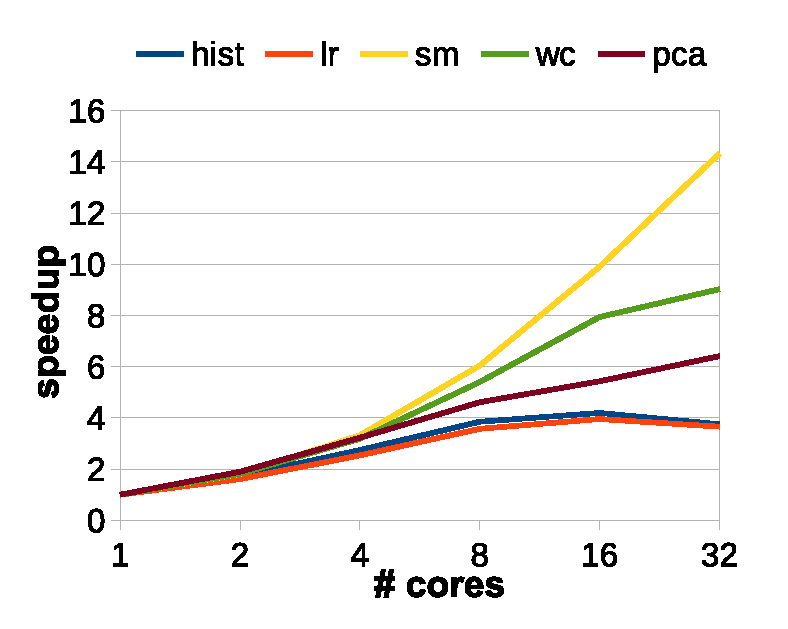
\includegraphics[width=0.45\textwidth]{eps/dmr_speedup.eps}
%		\label{fig:smr:speedup}
%	}
%	\subfigure[Execution time percent of \_\_tickect\_spin\_lock in \myds]{
%		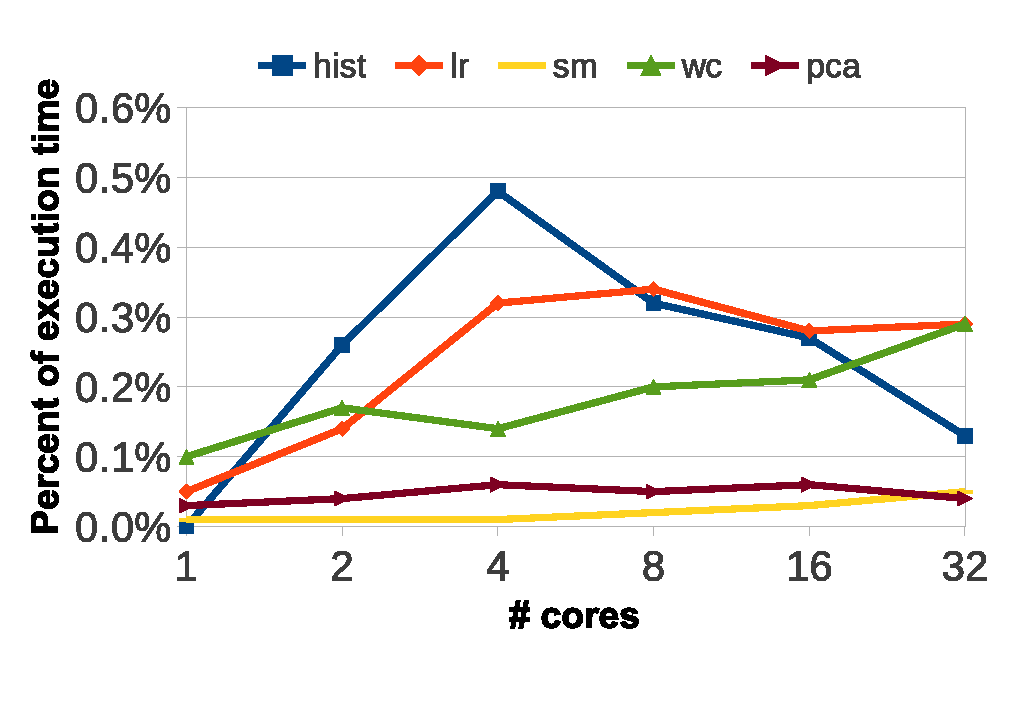
\includegraphics[width=0.45\textwidth]{eps/dmr_spinlock.eps}
%		\label{fig:smr:spinlock}
%	}
%	\caption{scalability of \myds}
%	\label{fig:smr:scalability}
%\end{figure}

Although with the scalable memory allocator, Phoenix can not scale up to 16cores.
 
\begin{figure}[!h!t]  
	\centering
	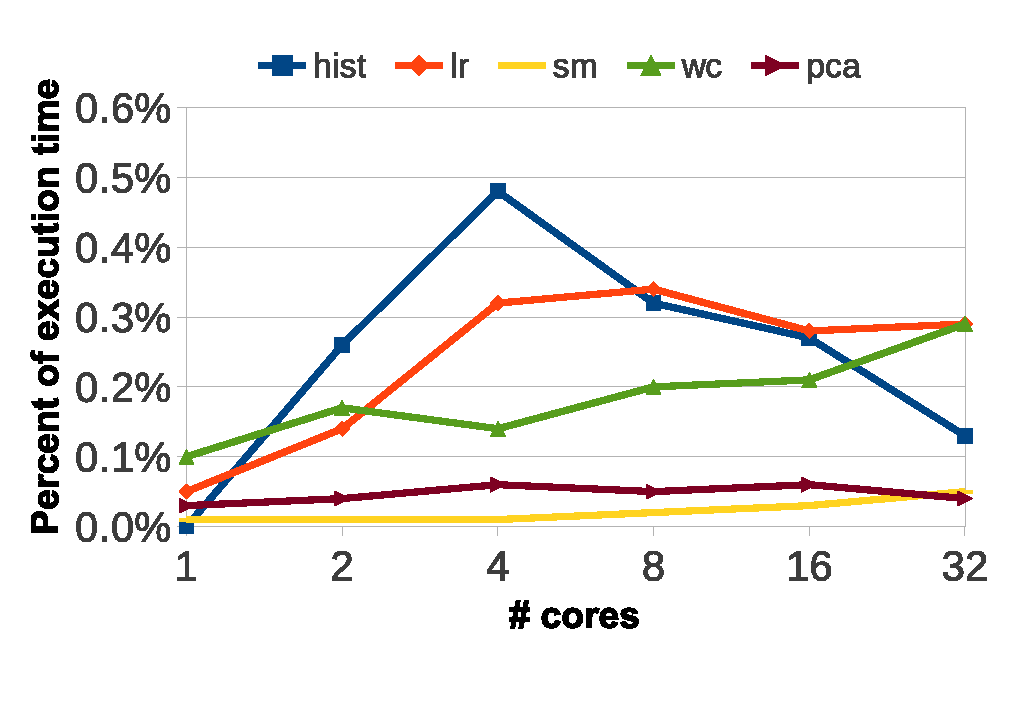
\includegraphics[width=0.45\textwidth]{eps/dmr_spinlock.eps}
	\caption{Execution time percent of \_\_tickect\_spin\_lock in \myds}
	\label{fig:smr:spinlock}
\end{figure}

Figure\ref{fig:smr:speedup} summarizes the scalability results for \myds.
Specially, workloads \codet{string\_match}, \codet{word\_count} and \codet{pca} scaled up to 32 cores.
And the performance of hist, wc, sm are scale linearly with the number of cores.
However, \codet{linear\_regression} and \codet{histgram} still did not scale particularly. 
We will discuss their bottlenecks in detail in subsection 5.4.
\begin{figure}[!h!t]  
	\centering
	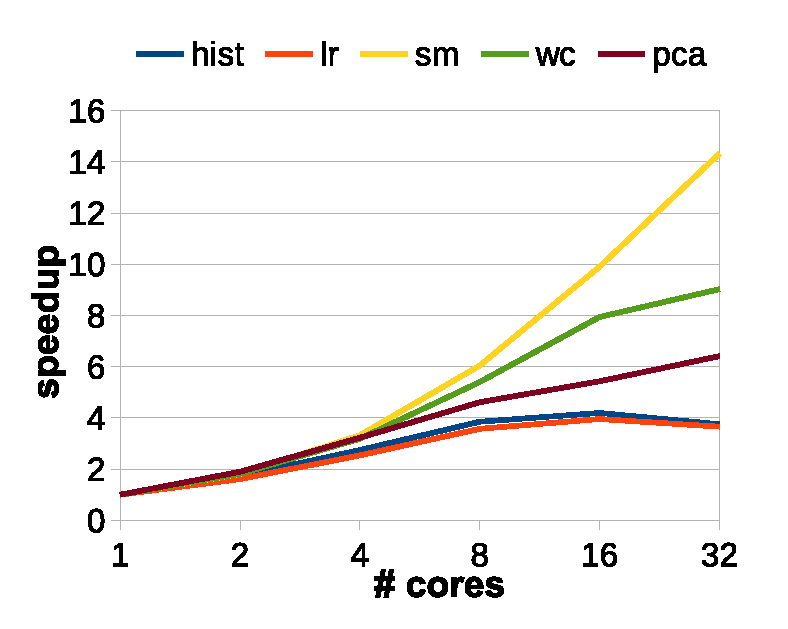
\includegraphics[width=0.45\textwidth]{eps/dmr_speedup.eps}
	\caption{speedup of \myds}
	\label{fig:smr:speedup}
\end{figure}

In our \myds, using \myth thread was sufficient to reduce the contention in Linux kernel. 
System Contention is evaluated using the execution time percent of \_\_ticket\_spin\_lock. 
Evaluation indicates (Figure\ref{fig:smr:spinlock}) that the locking overhead can be significantly reduced to less than 1\% of total runtime on 32 cores
%\begin{figure}[!h!t]  
%	\centering
%	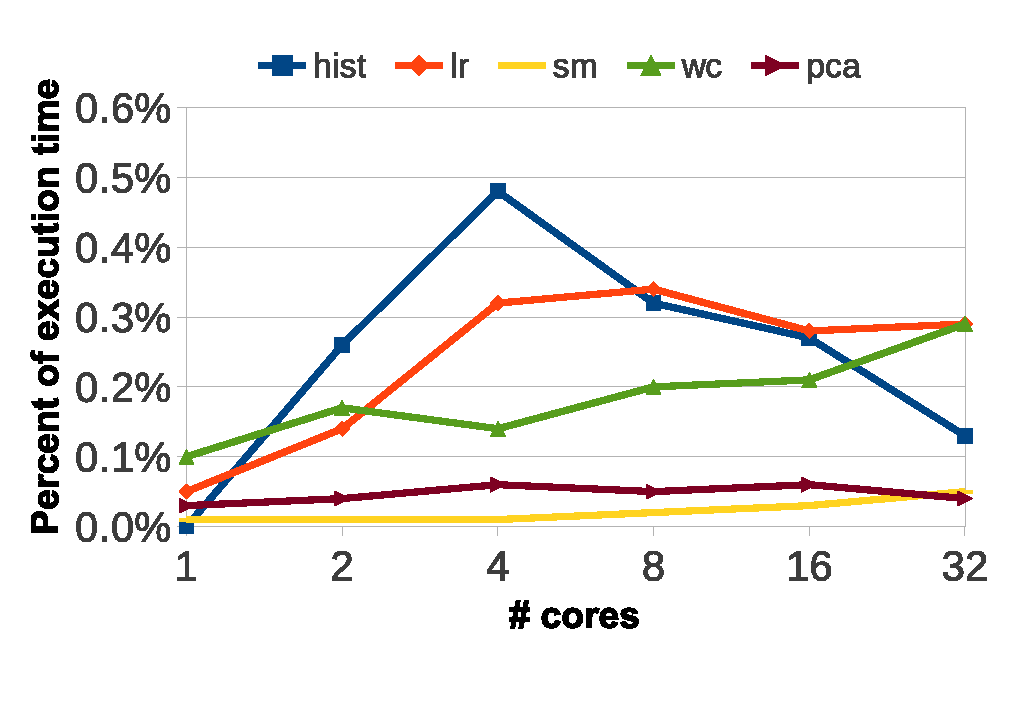
\includegraphics[width=0.45\textwidth]{eps/dmr_spinlock.eps}
%	\caption{tickect\_spin\_lock execution time percent of Phoenix}
%	\label{fig:smr:spinlock}
%\end{figure}

%We say a waiting thread is the thread which is waiting for shared
%data that produced by another thread. If using semaphore for
%synchronization, a waiting thread will be blocked and enlisted
%on the waiting queue by the OS scheduler. If using spinlock
%for synchronization, a waiting thread will do busy wait, i.e.
%spinning in a while loop. Embedded software applications
%that using semaphore to handle the synchronization could
%result in performance overkill, since it involves system calls
%translated into thousands of CPU instructions [1]; while using
%spinlock have problem of long busy-waiting time.

%When a running thread tries to read shared data,
%it must do busy wait until it has exhausted its time-slice
%or until another thread has withdrawn the occupation on the
%shared data. 




%System performance is evaluated using
%instructions per cycle (IPC). Higher IPC means
%better performance.
%Figure\ref{fig:perf:ipc} shows the IPC of Phoenix first increases 
%and then decreases as more threads are run on multi-core system.


To summarize, \myds demonstrated its performance and scalability for applications such as \codet{word\_count}, \codet{histgram} and \codet{pca}.
For applications such as \codet{linear\_regression}, \myds does not show its superiority, which we will analyze this result in detail in Section 5.4.

\subsection{ Impact of buffer Optimizations}
In Section 4.3, we discussed the organization of intermediate data is critical to the performance of many MapReduce applications.
Using the default hash buffer, need to gather the scatter key arrays together before sending them to the \codet{shared-channel}, which is time wasting.
we addressed this issue by providing a array implementation of buffer. 
Especially, array buffer, which is a continuous memory space, avoided buffer reallocation and coping.
However, not all the workloads benefited from the optimization.




%As described in Section 4.3, we provide two implementation of the local buffer in Map phase, i.e, hash buffer or array buffer.  
\begin{figure}[!h!t]  
	\centering
	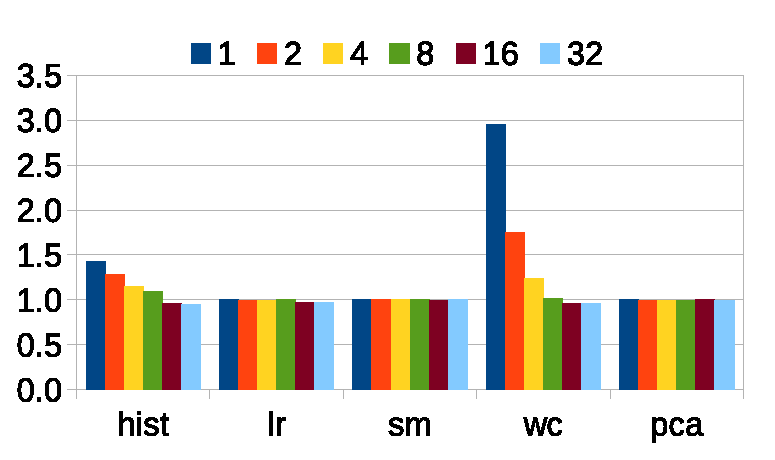
\includegraphics[width=0.45\textwidth]{eps/smr_diff_buffer.eps}
	\caption{Execution time of hash buffer over array buffer}
	\label{fig:smr:diff:buffer}
\end{figure}

%As the number of threads increases (from 1 to 8), the
%execution times for both Pthread/C and MPI programs decrease
%for both workstation and supercomputer. For 9 threads to 32
%threads, Pthread/C and MPI execution times changes slightly
%on workstation. However for 9 threads to 32 threads, both
%Pthread/C and MPI execution times keep decreasing (in most
%cases) with the increase in number of threads on the
%supercomputer node. This is because we use 8 cores in the
%workstation while we use 32 cores in the supercomputer node.
%Execution time for large number of threads (9 to 33 and
%beyond) remains almost the same for the workstation because
%of no communication overhead. Results (see Figure 4) also
%show that MPI execution time on supercomputer increases
%significantly when the number of threads is increased from 32
%to 33 and beyond; but Pthread/C execution time on
%supercomputer remains almost unchanged. This is due to the
%communication overhead among the cores (32 cores in a
%supercomputer node) when using MPI message passing.
Figure\ref{fig:smr:diff:buffer} shows the 
From the Figure, it can be seen that although cases such as \codet{word\_count} and \codet{histgram} used array buffer has better performance, other benchmarks, e.g., \codet{linear\_regression}, \codet{string\_match} and \codet{pca}, did not.
So, for workloads that did generate a large number of key-value pairs, gather operation in hash buffer waster more time, as a result, array buffer will be better.

From the experimental results, it is observed that benchmarks yield better performance using \myds than Phoenix (in most cases). 
\myds has the advantage over Phoenix for pipelining map and reduce phases and separating address space by using \myth thread instead of shared memory Pthread. 
The performance of the \codet{histgram} implementation on Phoenix is the best, 30\%-95\%x better than the Phoenix implementation on the our 32-cores system.

\subsection{ Challenges and Limitations}
Although we were able to significantly improve the scalability of \myds, 
workloads \codet{histogram}, \codet{linear\_regression} still did not scale up to 32cores (as shown in Figure\ref{fig:smr:speedup}). 
%We used /usr/bin/time to assess where the execution time was
We collect each phase time information to find out where the execution time was being spent by using stub. 
The results denote that workloads on \myds waste more execution time in initialization phase, compared to Phoenix.
Figure\ref{fig:env:init} shows the initialization time of \myds and Phoenix.
Exactly, the initialized time of \myds is range 0.25s to 0.35s, while it is just about 0.001s in Phoenix.
\begin{figure}[!h!t]  
	\centering
	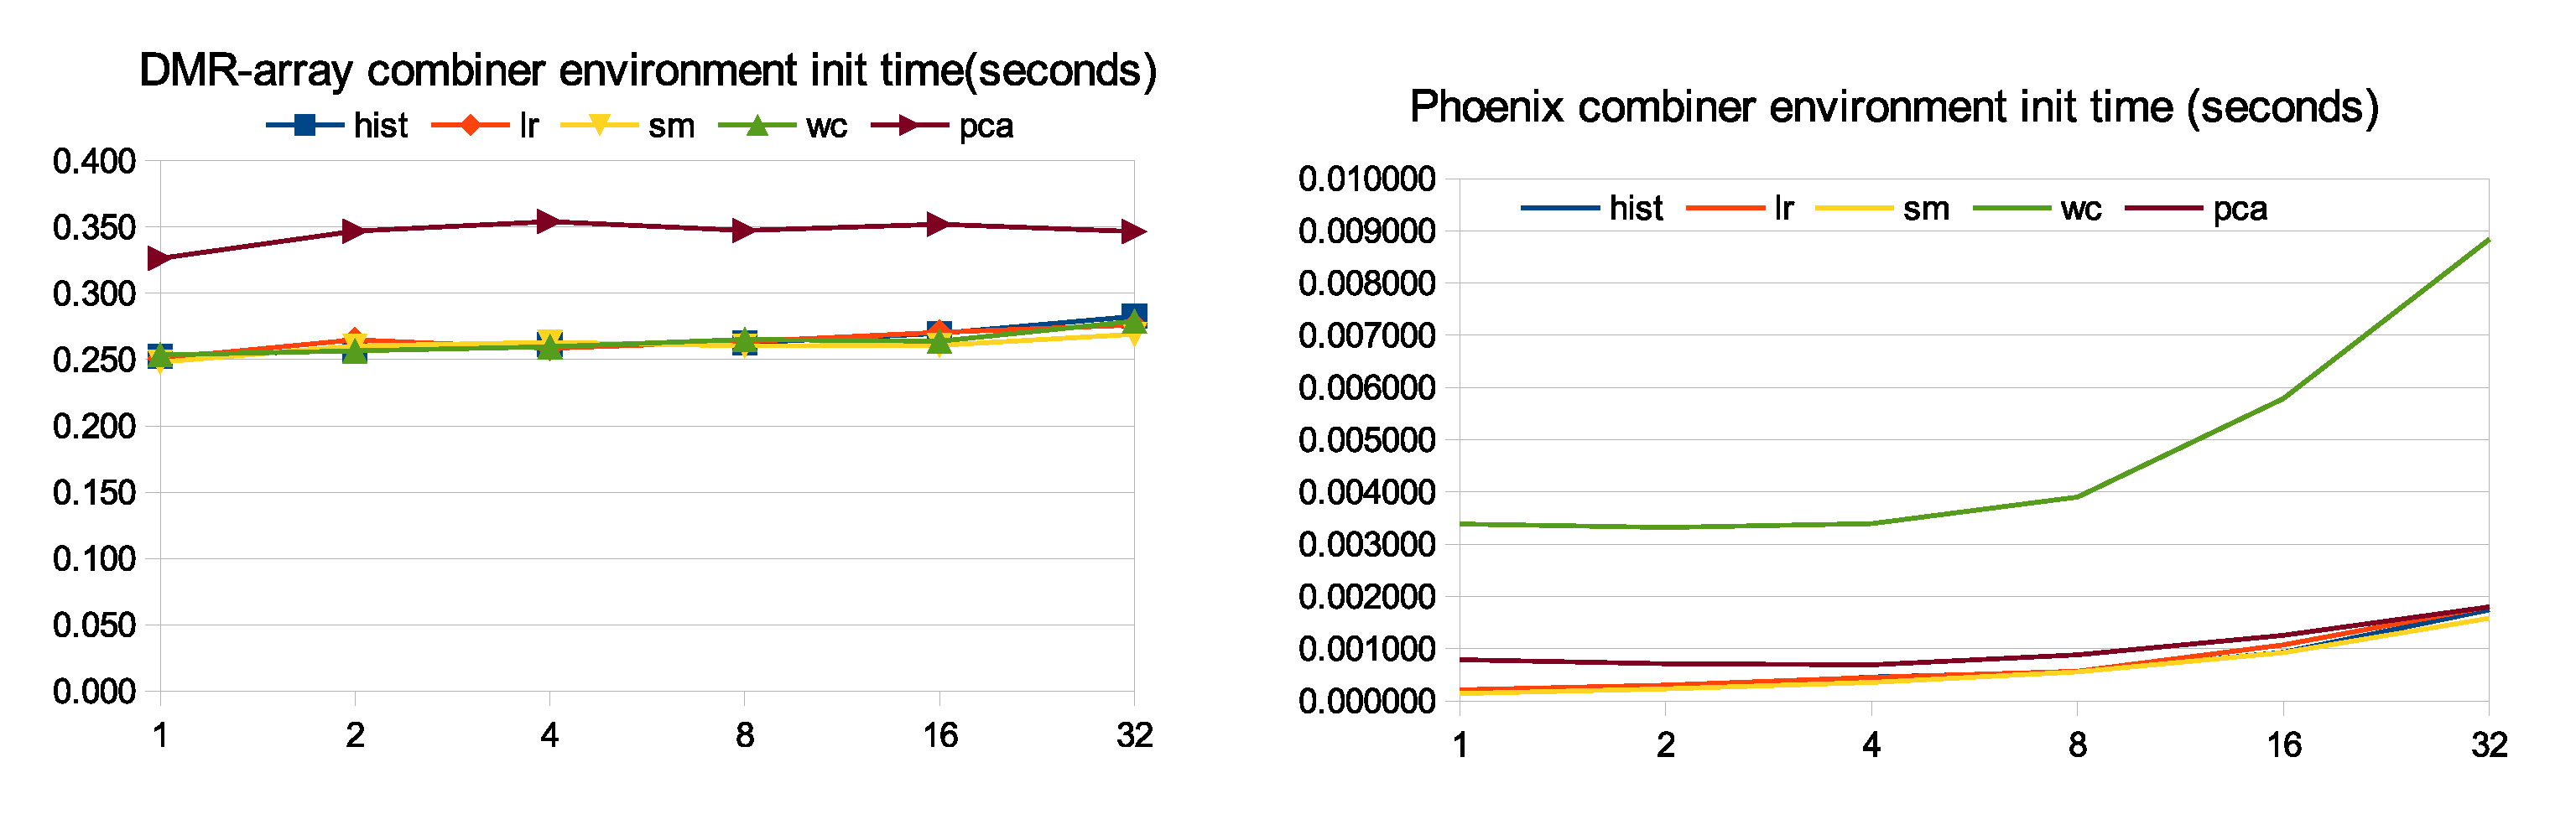
\includegraphics[width=0.5\textwidth]{eps/env_init.eps}
	\caption{initialization time of \myds and Phoenix}
	\label{fig:env:init}
\end{figure}


%解释为什么smr中的初始化时间会这么大
For multicore MapReduce library, most of initialized time is occupied in creating map and reduce threads.
Compared to thread in Phoenix, which based on Pthread, creating thread will spend more time in \myds because of more resource need to be allocated.
In addition, it will take more time for creating \codet{shared-channel} and setting up it.
From the experimental results (Figure\ref{fig:env:init}(b)), we observed that initialized time is small variation for different benchmarks and in different cores count, except for \codet{pca}.
Since there are two times mapreduce computation in \codet{pca}, which lead to two times initialization, it take more time than others benchmarks.
  

\begin{figure}[htpb]
	\centering
	\subfigure[Execution time and initialization time on histgram]{
		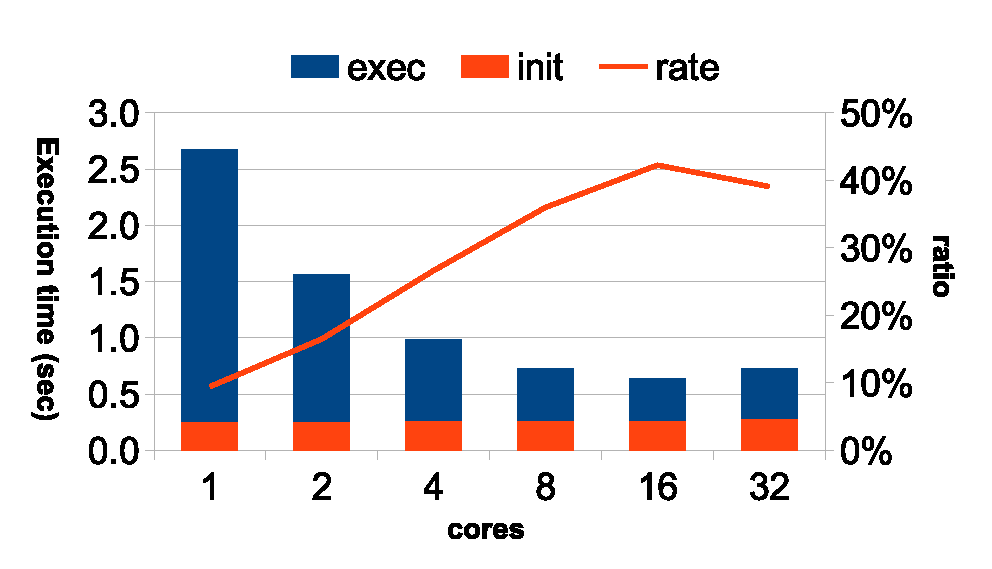
\includegraphics[width=0.45\textwidth]{eps/dmr_hist_init.eps}
		\label{fig:dmr:hist:init}
	}
	\subfigure[Execution time and initialization time on linear\_regression]{
		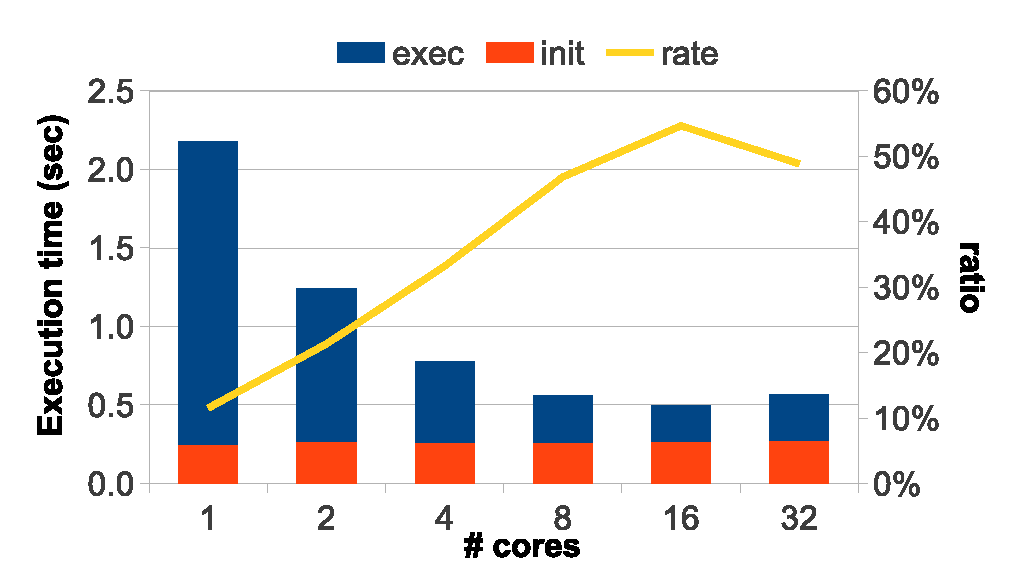
\includegraphics[width=0.45\textwidth]{eps/dmr_lr_init.eps}
		\label{fig:dmr:lr:init}
	}
	\caption{Initialize time with \myds}
	\label{fig:init}
\end{figure}


%这种较大较大的初始化对performance和scalability造成的影响


Figure \ref{fig:dmr:hist:init} shows the result with exec time defined as mapreduce actual execution time and init time as the initialization time before workers starting work. 
It was clear that the 2 non-scaling workloads shared two common trends. 
First, the total execution time of both \codet{histgram} and \codet{linear\_regression} less than 2.7s for all cores, which if far less than other benchmarks. 
Second, As the increasing number of cores, the portion of actual computation time (execution time) significantly decreased.
However, the initialization time is almost constant, which cause the init time ratio increase and dominate the total execution time at high cores count. 
As a result, the total execution time of \codet{linear\_regression} on Phoenix will less than on \myds.
%Second, the portion of actual computation time assumed by kernel code (sys /
%effective) significantly increased as we went beyond the single
%chip boundary.
%Second, both total execution time are short, While the portion of init time is 






\section{Related Work}
%两个方面:(1)面向多核的mapreduce的研究:Phoenix, mutis, MRPhi (2)linux scalability的问题
\label{sec:rel}
%在写这一部分的时候,需要将全部收集的论文重新看一边,并修改论文中的设计部分,最后,写好abstract, introduction, related work.

Our work is related to the research in programming models for
data-parallel applications, nested data parallelism and multicore re-
lated research. We briefly discuss the most related work in turn.
\subsection{MapReduce programming model}
MapReduce is a popular distributed framework
for massive-scale parallel data analysis.
There are many existing implementation of MapReduce 
which adopt on the basic architecture and 
programming model of originally Google's MapReduce, 
such as Hadoop\cite{}, Dryad\cite{isard2007dryad}.

The Phoenix MapReduce libray
is the most relevant work to \myds. 
Phoenix demostrate that MapReduce is a promising parallel programming
models in muliticore and multiprocess systems.
It creates a thread pool by Pthreads
and can schedule tasks dynamically to support itrative applications.
\myds differs from Phoenix mainly on that 
Phoenix need barrier between iterative MapReduce,
while \myds brokes barrier to speed up computing.

%虽然我们没有与mites, Tilt-MapReduce进行对比,但通过我们的研究,只要这些库使用pthread进行编程,那么就会存在scalability较差的问题。
Tilt-MapReduce\cite{chen2010tiled}
This paper argued that the environmental differences between
clusters and multicore open new design spaces and optimization
opportunities to improve performance of MapReduce on multicore.
Based on the observation, this paper proposed Tiled-MapReduce,
that uses the “tiling strategy” to partition a large MapReduce job
into a number of small sub-jobs and handles the sub-jobs itera-
tively. This paper also explored several optimizations otherwise im-
possible for MapReduce, to improve the memory, cache and CPU
efficiency.

Although, we don't compare \myds with mites, Tilt-MapReduce,
our research shows that if the MapReduce library implemented by Pthreads, there will be problem of scalability.

Metis\cite{mao2010metis},The paper’s main insight is that the organiza-
tion of the intermediate values produced by Map invocations and consumed by Reduce invocations is central
to achieving good performance on multicore processors.
Metis stores these intermediate values using an efficient
data structure consisting of a hash table per Map thread
with a b+tree in each hash entry. As a result, Metis can
achieve better performance than Phoenix on MapReduce
applications that interact with the library frequently (e.g.,
applications with many keys).

MRPhi\cite{} is a multicore mapreduce.

\subsection{Scalability of multicore}
A multicore operating system, named Corey\cite{boyd2008corey}, proposes three
new abstractions (address ranges, shares and kernel cores), to scale
a MapReduce application (i.e., Word Revert Index) running on Corey.
The work in Corey is orthogonal to Ostrich. The abstractions in
Corey, if available in commodity OSes, could further improve the
efficiency of Ostrich due to the reduced time spent in the OS kernel.
	
An Analysis of Linux Scalability to Many Cores \cite{Boyd2010An},
This paper analyzes the scaling behavior of a traditional
operating system (Linux 2.6.35-rc5) on a 48-core com-
puter with a set of applications that are designed for par-
allel execution and use kernel services. We find that we
can remove most kernel bottlenecks that the applications
stress by modifying the applications or kernel slightly.

RadixVM\cite{Clements2013RadixVM}RadixVM, a new virtual memory design
that allows VM-intensive multithreaded applications to scale
with the number of cores.



\section{Conclusions And Furture Work}
\label{sec:concl}
Phoenix shows MapReduce model is a promising model and approach to use multicore resource for multicore and multiprocessor systmes.
However, it has limitations in terms of scalability and performance due to its manners of design and implementation.

In this paper, we analyzed scalability and performance limitations of Phoenix and provide practicable solution.
we provide a novel thread programming model for support scalable mapreduce, i.e., \myds. 
We have presented \myds, a scalable MapReduce model for multicore system.
%to support efficient iterative processing.
We significantly improved the scalability over Phoenix, achieving an average speedup improvement of 2.5x, and a peek speedup improvement of 10x.
Our evaluation further shows the scalability and reliablity of \myds for iterative processing.
As to poor performance on multicast across processors, our future work will provide scalable iterative processing.
%\iffalse
%\section*{Acknowledgment} 
%{\small
%This work was supported in part by 
%the National High Technology Research and Development Program
%of China (863 Program) grant (No.2012AA010901),
%and the National Natural Science Foundation of China Grant (No.61170018).}
%\fi


\begin{small}
%\begin{footnotesize}
\bibliography{os,pa,my}
\bibliographystyle{abbrvnat}
%\bibliographystyle{plain}
%\end{footnotesize}
\end{small}

\end{document}
